% !TEX TS-program = pdflatexmk
% !TEX encoding = IsoLatin
%%%%%%%%%%%%%%%%%%%%%%%%%%%%%%%%%%%%%%%%%%%%%%%%%%%%%%%%%%%%%%%%%%%%

% University of Tampere
% School of Information Sciences
% Statistics

% A template for master's thesis and instructions for the use of the utastmth document class.

% Jarmo Niemel�, jarmo.niemela@uta.fi, 2014-12-31

%%%%%%%%%%%%%%%%%%%%%%%%%%%%%%%%%%%%%%%%%%%%%%%%%%%%%%%%%%%%%%%%%%%%
% This document uses a special document class utastmth, which defines the format of the document. Document class utastmth is based on the report class. The available options are oneside, twoside, draft, final, openany and openright. Default options are twoside, final and openany. Page size is always A4 (210x297mm) and font size is 12pt.
\documentclass[twoside]{utastmth} % see utastmth.cls

% The input character encoding is selected with the inputenc package. Here we use the ISO Latin-1 character set.
\usepackage[latin1]{inputenc}

% If parts of the thesis are written in Finnish, for example, use the babel package and its command \selectlanguage to select the Finnish hyphenation rules for those parts.
\usepackage[finnish,english]{babel}

% The packages amsmath and amssymb are always recommended if the document contains any mathematics, because they greatly expand the toolset for typesetting mathematics in LaTeX.
\usepackage{amsmath}
\usepackage{amssymb}

% Theorem-like environments are formatted with the amsthm package:
\usepackage{amsthm}

% According to university's graphic guidelines (http://www.uta.fi/hallinto/yliopistopalvelut/viestinta/avuksi/esittely/TaY_graafinen_ohjeisto.pdf) we use Times New Roman as serif font and Arial as sans serif font. If you don't have Arial fonts installed, you can use Helvetica fonts instead:
\usepackage[scaled=0.94]{uarial} % Arial text fonts.
%\usepackage[scale=0.94]{tgheros} % Helvetica text fonts.
\usepackage{newtxtext} % Times text fonts.
\usepackage[vvarbb]{newtxmath} % Times math fonts.
\usepackage{enumitem}
\usepackage{multirow} 
% As an alternative you can use LaTeX's default Computer Modern fonts. In that case comment out the previous three commands.
%\usepackage{lmodern}

% Bold math symbols, including bold italic letters, are accessed with the bm package:
\usepackage{bm}

% The graphicx package is needed for importing external graphics files.
\usepackage{graphicx}
\graphicspath{{Kuvat/}} % The relative path for the graphics files.
\usepackage{subfigure}
\usepackage{lipsum}

%\usepackage{pdfpages} % For including appendices as pdf-files.

% Table and figure captions are formatted with the caption package:
\usepackage[margin=\leftmargini, font=small, labelfont=bf, labelsep=period, tableposition=top]{caption}

% Author-year style citations and references are implemented with the natbib package. With the option longnamesfirst the first citation of any given reference is given with the full author list, but all subsequent ones with the abbreviated list, e.g. (Jones et al. 1990).
\usepackage[longnamesfirst]{natbib}
% Punctuation in citations is modified with the command \setcitestyle: 
\setcitestyle{semicolon,aysep={}}
% The format of the list of references can be modified:
\setlength{\bibhang}{\leftmargini} % indentation after the first line of each reference
\setlength{\bibsep}{3pt plus 1pt minus 1pt} % the space between references
\renewcommand*{\bibfont}{\small} % smaller font size for the references
% Natbib's command \bibsection must be redefined so that the page headers and/or footers will use the same style as other parts of the document. We also add the heading of the bibliography to the table of contents:
\renewcommand{\bibsection}{%
	\chapter*{\bibname\markboth{\bibname}{\bibname}}
	\addcontentsline{toc}{chapter}{\bibname}}
% If the same author or team of authors has several publications in the reference list, replace the name(s) with a long dash for second and subsequent works:
\newcommand*{\longdash}{---{}---{}---}

% Tables are formatted with the booktabs package.
\usepackage{booktabs}

% Computer program listings can be displayed with the packages fancyvrb and listings:
\usepackage{fancyvrb}
\usepackage{listings}
\lstset{literate={�}{{\"a}}1 {�}{{\"o}}1}
\lstloadlanguages{R}

% The following commands are needed for an index:
%\usepackage{makeidx}
%\makeindex

% The hyperref package turns LaTeX's cross-references into hypertext links. It also allows the user to write hypertext links to external documents and URLs. Hyperref should usually be the last package in the document.
\usepackage[hidelinks,pdfpagemode=UseNone,pdfstartview=FitH]{hyperref}
\urlstyle{same} % URLs are typeset with the same font as ordinary text.

% Theorems and lemmas are set in italic font:
\theoremstyle{plain}
\newtheorem{theorem}{Theorem}[chapter]
% Lemmas and theorems use a common numbering:
\newtheorem{lemma}[theorem]{Lemma}
% Named, unnumbered theorem:
\newtheorem*{Bonferroni}{Bonferroni inequality}

% Definitions and examples are set in normal upright font:
\theoremstyle{definition}
\newtheorem{definition}{Definition}[chapter]
\newtheorem{example}{Example}[chapter]

% Remarks are not numbered:
\theoremstyle{remark}
\newtheorem*{remark}{Remark}

% A square as a QED symbol is automatically appended at the end of a proof environment. This can be left out with the following definition:
%\renewcommand*{\qedsymbol}{\relax}

% A long chain of equations can be broken between pages:
\allowdisplaybreaks[1]

% The common number sets are depicted with the blackboard bold font:
\newcommand*{\Nset}{\mathbb{N}}  % the set of natural numbers
\newcommand*{\Zset}{\mathbb{Z}}  % the set of integers
\newcommand*{\Qset}{\mathbb{Q}}  % the set of rational numbers
\newcommand*{\Rset}{\mathbb{R}}  % the set of real numbers
\newcommand*{\Cset}{\mathbb{C}}  % the set of complex numbers

% Certain statistical operators are defined as LaTeX's mathematical operators. This improves their spacing in mathematical formulas (compare $P(A)P(B)$ with $\P(A)\P(B)$):
\DeclareMathOperator{\E}{\mathnormal{E}} % expected value
\DeclareMathOperator{\Var}{Var} % variance
\let\P=\relax % removing the previous definition of the command \P
\DeclareMathOperator{\P}{\mathnormal{P}} % probability
\DeclareMathOperator{\Gammaf}{\Gamma} % gamma function

\newcommand*{\ave}{\overline} % sample mean

% The documentation of the amsmath package (amsldoc.pdf pp. 16--17) recommends the following commands for absolute value and norm:
\newcommand*{\abs}[1]{\left\lvert#1\right\rvert}  % absolute value
\newcommand*{\norm}[1]{\left\lVert#1\right\rVert} % norm

% Matrices and vectors are denoted with the command \mx. If you want to use bold upright instead of bold italic, replace the command \bm with the command \mathbf. Be careful with the use of the command \mx, because it makes its whole argument bold. For example, don't write \mx{A+B} but \mx{A}+\mx{B}.
\newcommand*{\mx}{\bm}  % a matrix or a vector

% The command \sijoitus typesets the special symbol used (only?) in Finland when computing the antiderivative from a definite integral. For example, $\int_a^b 2x\,dx = \sijoitus{a}{b}x^2$. If you use this command, you should also use the amsmath option [intlimits].
\makeatletter
\@ifpackageloaded{newtxmath}

{\newcommand*{\sijoitus}[2]{\mathop{\bigg/}\limits_{\mspace{-9mu}#1}^{\mspace{9mu}#2}}}
{\newcommand*{\sijoitus}[2]{\mathop{\Big/}\limits_{\mspace{-19mu}#1}^{\mspace{19mu}#2}}}
\makeatother

% Normal inter word space is used after the end of a sentence:
\addto\extrasenglish{\frenchspacing}




%%%%%%%%%%%%%%%%%%%%%%%%%%%%%%%%%%%%%%%%%%%%%%%%%%%%%%%%%%%%%%%%%%%%
% Commands used only in this document:
\newcommand*{\BibTeX}{\textsc{Bib}\-\TeX}


%%%%%%%%%%%%%%%%%%%%%%%%%%%%%%%%%%%%%%%%%%%%%%%%%%%%%%%%%%%%%%%%%%%%

\begin{document}

% The sectional headings are not numbered at the beginning:
\setcounter{secnumdepth}{-2}

% The title page of the thesis:
\begin{titlepage}
\centering

\vspace*{\stretch{2}}


{\Large\bfseries Analysis and visualization of traffic signal performances}\\[2cm]
{\Large\bfseries Chenlu Wang}\\[1cm]
% The title should fit on three lines at most. Do not use hyphenation in the title, except between the parts of compound words. Break the lines with the command \\.
\makebox[0pt]{\large\bfseries }

\vspace{\stretch{5}}

UNIVERSITY OF TAMPERE\\
School of Information Sciences\\
Software Development\\
December 2015
\end{titlepage}

% When using the document class option twoside, the following page will be on the right hand side of the spread.
%\cleardoublepage


%%%%%%%%%%%%%%%%%%%%%%%%%%%%%%%%%%%%%%%%%%%%%%%%%%%%%%%%%%%%%%%%%%%%
% Model for the abstract

\begingroup
\setlength{\parindent}{0pt}
\setlength{\parskip}{\smallskipamount}
University of Tampere

School of Information Sciences

Wang, Chenlu: Analysis and visualization of traffic signal performances

Master's thesis, 50 p., 2 app. p. % Replace xx and x with actual page counts.

Software Development

December 2015\\
\rule{\textwidth}{0.5pt}
\endgroup

\section*{Abstract}

Road transportation network is significant backbone of current society with the increasing demand of mobility. Traffic controlling is a big challenge in many cities, especially growing cities.
Since the capacity of traffic throughput is limited in urban area, it is critical to improve the capacity of traffic network. Traffic signals controlling as an elementary component of all the road transportation system, it is used to solve this problem of traffic conflict on intersections.

However, many traffic management system is lack of the ability to qualify characterized arterial performances. That also provides the reason to develop methods to qualifying arterial performances.
The performance of traffic flow through intersections depends on the phases, sequence and the timing of traffic signals. Therefore, efficient traffic signal operation is vital for smooth traffic flows in signalized network, and well-maintained signal operation is greatly beneficial for road users. With the increasing traffic jam on the road, traffic engineers are looking for some new approaches on intuitive interface to manage and analyze the traffic signal system.

Traffic signals provide orderly and safe traffic movements at intersections, reduce the travel timing of vehicles passing through the intersections and balance the efficiency of management to all the traffic flows. It is difficult to identify the effects of any changes to the system without infrastructure to measure performances.Historically, many traffic engineers have made decision based on users' expectation and complaints, which is not a good practice.

Some traffic solutions provide measurements of traffic performance, like ImFlow system, which is a business product on European market.  ImFlow is professional but very high expenditures for equipment, installation and maintenance. Only 10 intersections have installed ImFlow system in Tampere.
The goal of my thesis is to develop a substitute of ImFlow that has no extra demand of equipment on roadway, as an economic and lightweight solution to satisfy the demand of performance analysis, further to assist traffic engineers manage and maintain traffic signal system in prevailing intersections.

In general, the common signal control system is consist of three types: the pre-defined type with fixed phases, vehicle actuated type which totally depends on the demand of vehicles and semi-actuated ones. The intersections equipped with detectors are said to be actuated, furthermore, an intersection with all approaches actuated is called full actuated and an intersection without detectors is called non-actuated or fixed. For saving money on maintenance, some intersections are set as semi-actuated.
A critical work for the thesis is to select suitable and useful measurements of signal performances based on available traffic data and engineers' requirements. The selected performances in the thesis include green duration, queue length, waiting time, volume, maximum capacity, saturation flow rate, active green and percentage of vehicle arrival on green. The algorithms used in the thesis are referred from others' previous research and adjusted based on our actual cases. According to measurements of those traffic performances, traffic engineers could make decision with analytical traffic data.


%There exists a Finnish standard SFS 3855 for writing abstracts. Below are some main points from it. Note especially that a short abstract should be written as a single paragraph, not as a list like the instructions here.
%\begin{itemize}
%\item The abstract should describe the content of the document briefly and clearly.
%\item The abstract should contain all the conclusions and the new information from the document.
%\item The structure of the abstract should follow the structure of the document itself.
%\item Finnish abstracts are usually less than 200 words long. The abstract should fit on one page and should contain no more than 400 words.
%\item The abstract should be independent and understandable without the original document.
%\item Use short complete sentences in the abstract. Short abstracts are written in one paragraph, longer abstracts can be broken into two or more paragraphs.
%\item It is preferable to use passive voice in the abstract.
%\item Do not use unusual abbreviations, symbols or terms without explaining them.
%\end{itemize}
%Do not use pictures, tables or complex mathematical formulas in the abstract, because the abstract is saved in electronic form as plain text.


\paragraph{Key words}
analysis, visualization, traffic signal system, signal performance measure


%On the same page with the abstract, you may optionally add three to six key words or phrases that do not already appear in the title of the thesis. The key words can describe the techniques used or the topic of the thesis, or they can be synonyms of the words and concepts in the title of the thesis. Key words should be exact and detailed rather than general. On the other hand, do not use any new or uncommon term as a key word. Do not incorporate several concepts into one key word. Do not use mathematical symbols and formulas. Use the singular rather than the plural whenever possible. More guidance on selection of key words can be found from the page \url{http://journals.taylorandfrancis.com/amstat/keywords-and-phrases/}.


% When using the document class option twoside, the following page will be on the right hand side of the spread.
%\cleardoublepage


%%%%%%%%%%%%%%%%%%%%%%%%%%%%%%%%%%%%%%%%%%%%%%%%%%%%%%%%%%%%%%%%%%%%
% The table of contents is placed here.
\tableofcontents

\listoffigures

\listoftables

% When using the document class option twoside, the following page will be on the right hand side of the spread.
%\cleardoublepage

% From this point onwards the top three sectional levels (0,1,2) are numbered:
\setcounter{secnumdepth}{2}


%%%%%%%%%%%%%%%%%%%%%%%%%%%%%%%%%%%%%%%%%%%%%%%%%%%%%%%%%%%%%%%%%%%%
\chapter{Introduction}

\section{Background}

The origin of traffic signal control can be traced back to the manually operated semaphores in 1868 used in London [\cite{STM:2008}]. Nowadays, the traffic signal control system has changed vastly since its early development.


Road transportation network is significant backbone of current society with the increasing demanding of mobility. Figure ~\ref{fig:daily volume of cities in Finland} from Finnish transportation agency demonstrates the average daily volume of cities in Finland and there are several cities occupying traffic volume over 30,000 per day. Traffic controlling and management is a big challenge in many cities, especially growing cities. Due to the capacity limitation of traffic throughput in urban area, it is critical to improve the efficiency of traffic network [~\cite{Chanloha:2012}]. Traffic signals controlling as an elementary component of all the road transportation system, is used to solve this problem of traffic conflict on intersections by time division multiplexing [~\cite{Aljaa:2014}].

The description of traffic performance on freeway in real time and based on historical data has been successfully achieved, however, the characterized arterial performance is still elusive and many traffic management and traveler information system is lacking of that kind of ability [~\cite{Wolfe:2007}], therefore it is quite meaningful to develop methods for quantifying arterial performance.

The performance of traffic flow through intersections depends on the phases, sequence and the timing of traffic signals.Therefore, efficient traffic signal operation is vital for smooth traffic flows in signalized network, and well-maintained signal operation is greatly beneficial for road users. With the increasing traffic jam on the road, traffic engineers are looking for some new approaches on intuitive interface to manage and analyze the traffic signal system. 
\begin{figure}
	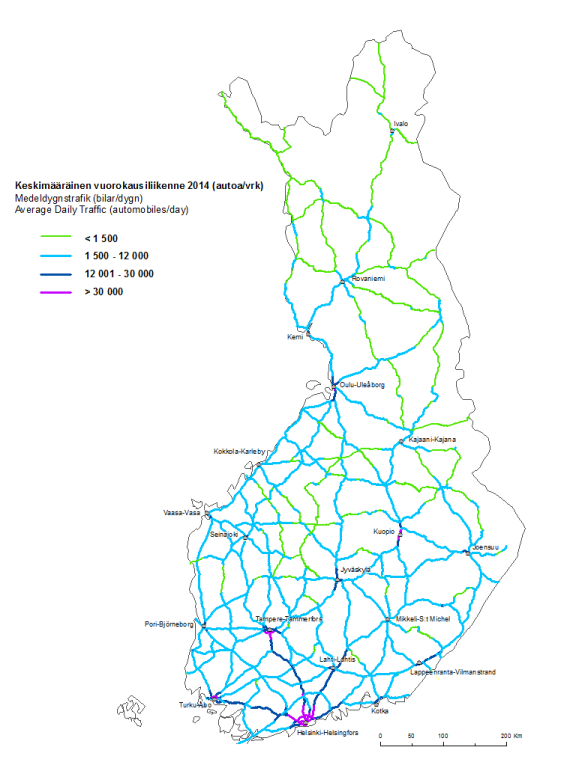
\includegraphics[width=1.0\linewidth]{finlandvolume.png}
	\caption{Daily volume of cities in Finland}
	\label{fig:daily volume of cities in Finland}
\end{figure}


\section{A statement of the problem}

In general, smart traffic controller systems aim to improve the efficiency of traffic control, save time for all drivers and pedestrians, make safe traffic.  How do the systems work? And can we know the way and efficiency of their work?  

In fact, raw data can be obtained from every controller. Unfortunately, most existing signal control systems do not make it convenient to monitor or archive traffic signal performance data. So far, the analysis tools which could analyze the raw data to present concrete traffic signal controlling is appealing and necessary. In addition, it would tell the engineers if signal control system operates as it should be in design. 

On the other hand, general road users and stakeholders cannot access and analyze traffic signal raw data as which usually is not open data. Sometimes there is a poor understanding of the relation between settings in use and their effects on operation. Historically, many traffic engineers have made decision based on users' expectation and complaints, which is not a good practice [~\cite{STM:2008}]. Based on the performance measured by the analytical application, users can easily gain comprehensive decision making help and look over the traffic condition without any programming or statistics background. With the analysis application, it is quite helpful for operators to build a context sensitive approach with consideration of the environment of traffic signals, location conditions and unintended consequences of potential changes[~\cite{STM:2008}]. 

Signal timing is complicate because operators cannot have a clear vision to insight the ongoing behaviors of the entire traffic signal system. Traffic signal operation is more complex than freeway operation, because it is difficult to identify the effects of any changes to the system without infrastructure to measure performances [~\cite{STM:2008}].

There are some traffic solutions providing the analysis of traffic performance. ImFlow is one of products on market from the company Imtech Traffic \& Infra, offering understandable policies and constraints to traffic engineers who need to setup and maintain the Imflow system. The policies and constraints are directly entered into the system and can be used by adaptive algorithms to optimize the signal timing in real-time and also collect some historical data. ImFlow central is a web-based system for monitoring and controlling of DAAP devices. According to ImFlow central, users can interact with ImFlow using a web browser, configure tools and display setting for the best performance. The performance reports are available, which include signal performance, PT Route performance and route travel performance [\cite{ImFlow:2014}]. 

However, due to the high requirements, expenditures for equipping hardware of ImFlow and other reasons, only a few intersections are deployed with Imflow system in Finland. Take the city of Tampere as an example, currently ImFlow is valid in only ten intersections distributing on Satakunannkatu and H�meenpuisto. Whereas, for the rest of hundreds intersections in that city, no specialized service about traffic performance measurements and analysis is provided to traffic engineers.

Therefore, it is necessary to develop a substitute that has no extra demand of equipment on roadway, as an economic and lightweight solution to satisfy the demand of performance analysis, further to assist traffic engineers manage and maintain traffic signal system in prevailing intersections. 

The aim of this thesis work is for traffic engineers to provide understandable report in prevailing intersections to present the behavior of traffic signal controllers, evaluating the performance of smart traffic system and integrate the various analysis models into a interactive web service for multi-dimensional measurements and continuous monitoring of traffic performance.  The analysis service is given the name ImAnalyst as a product of Imtech traffic \& Infra Oy.

\section{The definition of terms}

This application involves a lot amount of terminologies about traffic signal regulations and road rules. The relevant terminologies with their definitions and brief explanation are listed alphabetically as following.

\renewcommand*{\descriptionlabel}[1]{\normalfont #1\ }

\begin{description}

\item[\texttt{Actuated operation}]
All the traffic signal controlling operations are actuated from the vehicle detectors.

\item[\texttt{Approach}] 
A set of lanes at an intersection that accommodates all left-turn, through, and right-turn movements from a given direction.

\item[\texttt{Arrival rate}]
The mean of a statistical distribution of vehicles arriving at a point or uniform segment of a lane or roadway [\cite{STM:2008}]. 

\item[\texttt{Arterial}] 
A signalized street that primarily serves through traffic and that secondarily provides access to abutting properties with signals [\cite{HCM:2010}].

\item[\texttt{Capacity}]
The maximum number of vehicles can pass over a specified roadway or section of roadway expectedly in a direction, during a certain time period. 

\item[\texttt{Critical lane group}]
 The groups of lanes that have the highest flow ratio for certain signal phase [\cite{HCM:2010}] .

\item[\texttt{Critical volume}]
A volume produces the largest utilization of capacity on a road, and it measures the number of vehicle can pass over per hour per lane. 

\item[\texttt{Cycle}]
One complete sequence of the indication of traffic signals. Cycle time or cycle length is the time taken one cycle. The cycle length controls the time from one intersection green to the next intersection green. It is often pre-set by the particular plan used. 

\item[\texttt{Detector}]
The sensing equipment that requests or extends on a specified traffic and pedestrian phase. It includes the loops buried or above the carriageway and some other kind of detectors. 

\item[\texttt{DINT}] The code representing the status of detectors using in the traffic flow garner system.

\item[\texttt{Downstream}]
The direction of traffic flow [\cite{STM:2008}] .  

\item[\texttt{Flow rate}] 
The equivalent hourly rate at which vehicles, bicycles or persons pass a point on a lane, roadway or other traffic way; computed as the number of vehicle, bicycles or persons passing the point, divided by the time interval in which they pass. 

\item[\texttt{Gap, extension or passage time}]
Passage time determines the extentable part of the green timing for a movement.Take an example, assume the passage time is 3 second, and no vehicles pass after 3 second, the movement should terminate[\cite{wiki:Signaltiming}].

\item[\texttt{GRINT}] The code presenting status of signal group using in the traffic flow garner system.

\item[\texttt{Headway}] 
The time in seconds between two successive vehicles as they pass a point on the roadway, measured from the same common feature of both vehicles (for example, the front bumper).

\item[\texttt{Intergreen period}]
The time between end of a green phase and start of the next green phase for another. These comprise of several seconds amber for the phase losing right of way and several second amber/red for the phase gaining right of way. The all red might occur to allow clearance depending on the geometry of the intersection. 

\item[\texttt{Loop detector}]
The inductive loops embedded on the road surface relying on the electromagnetic change to detect vehicles passing over.

\item[\texttt{Maximum green}]
The maximum duration of a green signal after a conflicting demand has been registered in the controller

\item[\texttt{Minimum green}]
The minimum green during green signal time no change of the signal lights can occur.

\item[\texttt{Movement}] 
Movement is an item to describe the user type(vehicle or pedestrian) and action (turning movement) taken at an intersection. Two different types of movements include those that have the right of way and those that must yield consistent with the rules of the road or the uniform vehicle code [\cite{HCM:2010}].

\item[\texttt{Offset}]
The time difference between a certain point in a cycle and a reference point at an intersection.

\item[\texttt{Passenger car unit}]
A unit for measure the number of vehicles consideration the large trucks and turning movements using multiplication factors. It allows you to handle mix traffic streams more accurately than just assuming all the vehicles are same. 

\item[\texttt{Peak hour}]
The hour of a day that obverses the largest utilization of capacity or when there is largest number of vehicles use the traffic approach or lanes.

\item[\texttt{Pedestrian crossing time}]
Pedestrian crossing time serves on the green time allocated to each phase of a cycle.it is the sum of green interval and inter-green interval.

\item[\texttt{Platoon}] 
A group of vehicles or pedestrian traveling together as a group, either voluntarily or involuntarily because of signal control, geometrics or other factors.[\cite{HCM:2010}]

\item[\texttt{Pre-timing operation}]
All the traffic signal operations follow a fixed sequence, signal cycles with fixed length.

\item[\texttt{Queue}]
A closing space collection of vehicles nearby intersection stop bar. 

\item[\texttt{Queue discharge}] 
A flow with hight density and low speed, in which queued vehicles start to disperse. Usually denoted as Level of Service F.[\cite{HCM:2010}]

\item[\texttt{Right of way}]
The right to move for a traffic movement in a particular direction.

\item[\texttt{Saturation flow}]
The maximum flow during the green time from discharging queue. It is usually indicated by vehicle or passenger car unit per hour. 

\item[\texttt{Semi-actuated operation}]
The intersection is programmed to operate a fixed time every cycle, until there is a demand from some particular movements. 

\end{description}

In addition, for understanding the research well, some other traffic conventions in Finland are needed to learn.

Firstly, as for data naming, names of intersections often are combined with a prefix standing for the city and a index number. For example, the intersection ''TRE306'' starts with ''TRE'' means that it is NO.306 located in city of Tampere. 

Secondly, names of signal groups are letters of alphabet, what worth noting is that the signals for pedestrian always start with an underscore to distinguish with signal of vehicles, like {\_}G and {\_}K. 

Last but not least, since there are many different kinds of detectors with various significance, it is helpful to understand the type of a detector from its name. In general, inductive loop is the most common and widely-used detectors organized in different sizes and shapes, whose name is always starting with the upper case letter of signal group and a number meaning the distance between the detector and intersection stop bar, for instance, ''B100'' means that the detector belonging to the signal group B with 100-meter distance. Besides, ''A60{\_}1'' and ''A60{\_}2'' indicate that at the place located with 60-meter distance from the stop line, there are two paralleled detectors on the two lanes under the controlling of signal A.

\section{Technical background}


\begin{figure}[h!]
	\hspace*{.5in}
	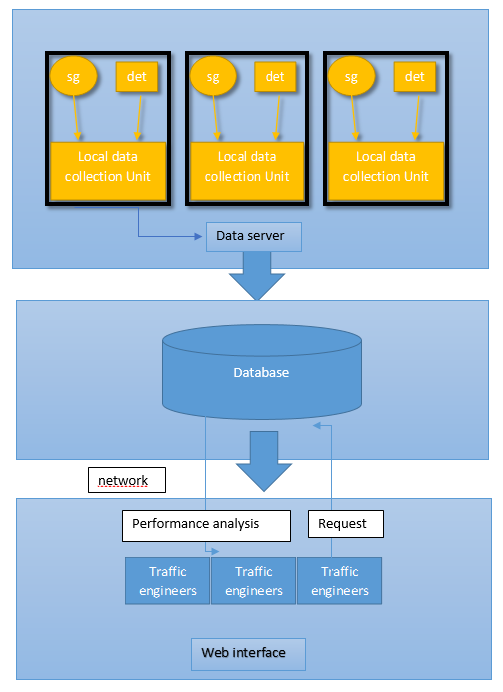
\includegraphics[width=0.8\linewidth]{flowchart.png}
	\caption{System flow chart}
	\label{fig:flowchart}
\end{figure}

The development procedure of the entire system are illustrated in figure ~\ref{fig:flowchart} which is mainly divided into three steps, simply summarized as: traffic signals data collection, storage and analysis. The research work of this thesis focuses on the last part: analysis and visualization of traffic signal performances. A practical scenario is that traffic engineers send analytical requests via web browsers to the server, and data retrieved from database using the parameters on users' submission, then the computation is processed on the back end of the server. After it is done, the analysis results will return to users and render on the web interface in a proper way.  


\subsection{Source of the study data}

 The first critical step to achieve the goal of research is obtaining data. As it is illustrated in the first block of figure ~\ref{fig:flowchart}, once any status of signal group and detectors updates, the data collection unit of local controlling gets the message. According to a serial port communication, these messages are synchronous and provide consistent data flow to the data garner system. Then the TrafficFlowGarner system, which is another application been used handles the incoming data by itself and store it into database [~\cite{TFG:2015}] . 
 
\subsection{Development environment}

\subsubsection{Production components}

\begin{itemize}[label=-]
  \item Python: The traffic signal analysis named ImAnalyst is implemented as an interactive web application using Django web framework written in python.
  \item Django: Django is a free and open source framework following model-view-controller (MVC) architecture, encouraging rapid development and clean, pragmatic design.  
   \item PostgreSQL: PostgreSQL is the supported database of this production as it is used by TrafficFlowGarner system as well. It is an object-relational and open-sourced database management system to store data securely, supporting very good practice and allowing the retrieve at the request from other software applications. 
   \item Git: Git is used as the version control system of the project during development.
\end{itemize}


\subsubsection{User interface components}

\begin{itemize}[label=-]
  \item Template: Django templates contains the static parts of the desired HTML, and the dynamic content can be inserted into the template with some special syntax in Django template language.  
  \item Static assets: Within the template, static files are referred with template tags. The system uses CSS, JQuery and JQuery assisted UI components to build HTML.
   \item Bootstrap:  Bootstrap is a twitter-style web framework.
\end{itemize}

\subsubsection{Development components}

\begin{itemize}[label=-]
  \item Anaconda: Python distribution to have almost all required packages in one.Due to the huge demand of data processing and analysis, Anaconda environment is used for simplifying package management. It is a python distribution having almost all the required packages for large scale data processing, analytics and scientific computing. 
  \item LiClipse: Lightweight editors for Python development. It is possible to use other IDE as well.
\end{itemize}

\subsubsection{Key parts}

\begin{itemize}[label=-]
  \item Middleware: Authentication of the project is controlled by a common middleware component. Only if the users whose IP addresses are included in the allowed ip range of network can access the application. The allowed network set is defined in the settings file.
  \item Django session: Django session provides a ''per-site-user'' solution.  Request session is used to pass values between different views and please ensure 'SessionMiddleware' is activated. Besides, GET request and POST request also pass values in views.
   \item User permission: Users' identification and authentication are performed in the middleware, which decides whether a user is able to access the application or not. The range of intersections that users could access is specified. The mapping of IP address and intersection naming is also defined in setting file.
   \item Database: The system connects the database of traffic flow garner system. Traffic flow garner system is used to collect and store traffic signal controlling data into database. The configuration of database connection is done in the settings file of the project. To retrieve data, the system handles database using raw SQL queries in Python code. And another way is to perform database using Django models. Alternatively, do database work in database is also OK, for example, using filter and exclude to filter database.
\end{itemize}



\section{Thesis organization}
The thesis is separated into the following sections:

\begin{enumerate}
	\item Fundamental of traffic signal controlling
	\item Analysis and visualization of traffic signal performances
	\item Validation and evaluation of traffic signal analysis
	\item Discussion
	\item Conclusion
\end{enumerate}

Each of the sections is subdivided into several aspects, many of which are discussed in more than one sections. In the chapter ~\ref{ch: fundamental of traffic signal controlling}, the basic operation principle of traffic signal controlling is introduced and some previous work and related algorithms are mentioned. The original work are presented in the chapter ~\ref{ch:The analysis and visualization} , then evaluation of reliability and accuracy of those measurements is done in the next chapter ~\ref{ch:Validation of evaluation}. 


%%%%%%%%%%%%%%%%%%%%%%%%%%%%%%%%%%%%%%%%%%%%%%%%%%%%%%%%%%%%%%%%%%
\chapter{Fundamental of traffic signal controlling}\label{ch: fundamental of traffic signal controlling}

Traffic signals provide orderly and safe traffic movements at intersections, reduce the travel timing of vehicles passing through the intersections and balance the efficiency of management to all the traffic flows [\cite{Trafficsignal}].  In an ideal condition, the signal control system should allow all the vehicles passing without stops, that means, phase transitions organizes a green band through all the intersections for each vehicle from the starting point to the destination. While, in fact, such control system is impossible to implement. 

In general, the common signal control system is consist of three types: the pre-defined type with fixed phases, vehicle actuated type which totally depends on the demand of vehicles and semi-actuated ones[\cite{List:2004}]. The intersections equipped with detectors are called ''actuated'', furthermore, an intersection with all approaches actuated is called full actuated and an intersection without detectors is called non-actuated or fixed. For saving money on maintenance, some intersections are set as semi-actuated [\cite{wiki:Signaltiming}].


\section{Signal timing operation}

\cite{wiki:Signaltiming} defines signal timing as the technique that traffic engineers used to determine the right of way at intersections, the during of green for vehicles and pedestrian walk, and many other related factors. In addition, cycle length is defined as the time from one main street to the next main street for coordination.

As \citet*{FHWA:signaltiming} suggests, all the signals that are synchronized together must operate the same cycle timing. Generally, the longest cycle length demand would be used. However, if there are three synchronized intersections requesting 75,80 and 80 seconds cycle length separately, the 80-second cycle length should be operated. In a word, a common cycle length is significant to operate coordinated signals. The classical approach to determine cycle length provided by Webster is expressed in the  equation ~\ref{eq:cycle length}:

\begin{equation}\label{eq:cycle length}
C =(1.5\times L)\div(1.0-Y_{i})
\end{equation}

where, $C$ is optimum cycle length in seconds, and cycle lengths in the range of 0.75$C$ to 1.5$C$ do not increase much delay. $L$ represents the lost timing per cycle in seconds and $Y_{i}$ is sum of the saturation degree for critical phases[\cite{FHWA:signaltiming}].

\section{Study of Queue at intersections}
Two typical and primary measures of performance of intersection is queue length and delays, with associated with frequent stops caused at intersections. The queue length is a good quantification for the performance of an intersection. The number of vehicles in the queue and associated delay is worthy to be calculated for improving and inspecting the traffic management strategies[\cite{Anusha:2013}].

Estimation of queue length is a long-standing issue. The traditional approach is to handle it by input-output traffic flow, which works well with the queues shorter than the distance from the selected detector to intersection stop line [\cite{liu2009real}]. The another method is to use traffic shockwaves to calculate queues.  As byproducts of traffic congestion and queueing, shockwave are traveling disturbance between two traffic states[\cite{Trafficwave}]. 

The widely and commonly applied sensors are loop detectors in Finland for detecting vehicles automatically. The loop detectors will return a pulse when any vehicle pass over it. The value of digitalized pulse is higher than the pre-setting threshold of the detector when vehicle passed and ideally equals to zero when no vehicle passing on [\cite{Anusha:2013}]. In reality due to existing noise, the pulse could be slightly higher than zero and sufficiently lower than the threshold. 

Webster F. asserts in his book Traffic signal settings, a traditional method to estimate queue length at signalized-intersection that is to analyze the cumulative traffic input and output [\cite{liu2009real}]. The Input-Output model is based on the difference between the total arrivals and the total departures, which has obviously drawbacks. Firstly, it could just handle queues that are shorter than the length between detectors and intersection stop line [\cite{liu2009real}]; second, it is too dependent on the accuracy of traffic flow measurement. Last, it requires the initial number of vehicles which is hard to obtain from loop detectors [\cite{Anusha:2013}].  

\cite{Ska:2008} designed an analytical model for real-time estimation along arterials, which compares the estimated travel times with simulated data to predict travel time on selected intersections.They proposed a method that using aggregated loop detector data in 30-second time interval to  estimate queue length at intersections.

Liu et al. created an algorithm using shockwave theory to estimate the queue length in intersection even when the road is congested with a queue which length is longer than the distance from intersection stop line to advance detector. This algorithm is relatively complex that requires to calculate multiple shockwaves and identify ''break points'', and their model utilize the break down points (A, B and C) identified using high resolution. Finally, based on identification of the break points, to make a decision to select methods for event-based data, second-by-second data and wired detector data separately [\cite{liu2009real}]. The approach asserted by Sharma et al. is suitable to estimate the queue length at intersections under low volume conditions. In their research, they observe the actual number of vehicles entering and exit manually using video. The accuracy of the approach to estimate queue length is shown in the Figure ~\ref{fig:queue polygon} estimated by queue polygon method [\cite{Anusha:2013}] .

\begin{figure}
	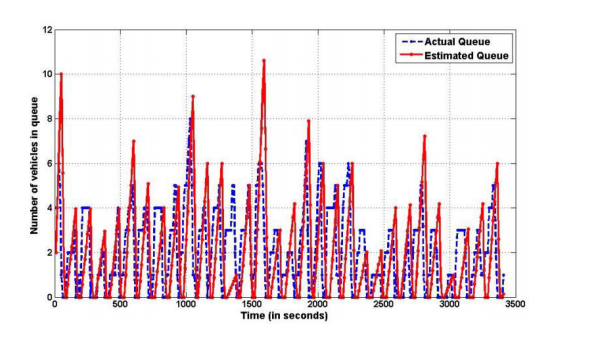
\includegraphics[width=\linewidth]{1.png}
	\caption{Queue estimated by the queue polygon method }
	\label{fig:queue polygon}	
\end{figure}

The algorithm of queue polygon processes input such as exit detector actuations and signal timing information. At the end of every cycle. It estimates the queue length for the previous cycle. The required signal timing information includes the cycle start time, end of red and end of green for every cycle. The key of the queue clearance time is figuring out a ''cut-off point'', when the queue actually gets clears. Thus, the vehicles after the queue clearance timing arrive the entre detector can pass the intersection without delay and stops.  

In the traffic analysis tool, the number of vehicles passing over specified intersection and detector in every cycle from the end of green time to the end of red time will be calculated. 

\section{Delay at signalized intersections}

Vehicle delay is a very important roadway traffic metrics in evaluating the performance of traffic signal controllers. Delay at intersections is usually difficult to be determined because the arrival and departure process is non-deterministic, which might be caused by the existence of traffic signals, the signs and the crossing traffic [\cite{doi:10.3141/2130-14}]. 

 However, there are many models using some assumption to simplify the complex issue. Delay can be estimated with the knowledge of arrival rate, departure rate and red timing. Delay at an intersection also can be approximately treated as all the extra time that a vehicle spends at the intersection comparing the time it should pass without any hindrance. The total delay includes deceleration delay, stopped delay and acceleration delay.  

\cite{doi:10.3141/2130-14}supposed a delay pattern to estimate the delay for any vehicle at any timeof a day at the intersection. Most existing delay models need the knowledge of traffic signal timing and traffic volume to estimate intersection delays. However, their model does not require signal timing data,only some sample travel time between two consecutive location on the street between upstream and downstream of the intersection. The two-step algorithm is: firstly, as the delay curves are piecewise linear (PWL) curve,delay measurements can be fitted by linear forms and fit a simple curve fitting algorithm. In addition, handle the increase in delays right after the start of the red time.

\section{Research on saturation flow rate}

Accurate saturation flow rate is a vital fundamental in urban traffic signal controlling management and design.Many factors lead to the different saturation flows on the roads. Influence of those factors includes: 

\begin{itemize}
	\item A multitude of different kinds of vehicles on the road with different performances,such as buses, trucks and ambulance. The heavy vehicles may influence saturation flow rate decreasing in two ways: They keep longer headway and also increase headways of other passenger cars. 
	\item Driver behavior varies based on personalities and traffic rules.
	\item Roadside activities like parking and non-transport activities which effect road condition.
\end{itemize}

Under ideal conditions, during the signal showing green, firstly there is a short gap as the first vehicles react to move, then the queue of vehicles could reach a state where they passing stop line one by one in a constant gap or headway.The last vehicles in the queue are supposed to be slow down at the end of green timing to red period[\cite{Turner:1993}]. Thus, \citep*{HCM:2010} suggests a way to estimate saturation flow rate by recording the time of passage of the fourth and tenth vehicles to determine the value based on the assumption that the initial queue at the end of previous red period is not less than ten vehicles. 

The first and last few vehicles are excluded because of they suffered from losing green time. In the thesis work, this approach proposed in Highway Capacity Manual was applied to calculate saturation flow rate.From queuing theory, the vehicles in a queue will discharge at the saturation flow rate and we can take advantage of the average headway of the vehicles and convert it to saturation flow rate. For instance, if the stable headway is two seconds per vehicle in average, in other words, every vehicle requires 2 seconds of the effective green, the saturation flow rate of this lane is 1800 vphgpl(vehicle per hour of green per lane).

For general calculation purpose, there are the studies about movements of vehicles at an intersection by Greenshields. Greenshieds found that the first vehicle enters an intersection with 3.4 second delay, while subsequent vehicles take 2 to 2.5 seconds in average to pass over a detector when considering the headway between vehicles [\cite{idaho:1995}].

 \cite{Turner:1993} proposed several methods to collect saturation flow data for estimating saturation flow and using multiple linear regression to build predictive saturation flow models.The basic idea is to use timekeeper and record the number of vehicles in every 6-second interval as Method 1, where the start period sets to 10 seconds as Method 2 and one where the start period equals the time for 3 vehicle to depart is Method 3. Their conclusion is that the method 2 gives the most appropriate result. 
 
 Due to the traditional method might lead to underestimated results, \cite{Shao:2012} provides an approach to study stochastic nature of queue discharging headways and to develop a model to estimate the saturation flow rate based on the surveyed data set. They found that the queue discharging headway is fitted in lognormal distribution and its density function ~\ref{eq: the lognormal distribution density function of headway density} is: 
 
 \begin{equation}\label{eq: the lognormal distribution density function of headway density}
 f_{H}(h) = \frac{1}{\sqrt{2\pi}\delta h}exp(- \frac{(lnh-u)^{2}}{2\delta^{2}}), h\geq 0
 \end{equation}
 
 The traditional way to calculate saturation flow rate is as the equation ~\ref{eq:use mean value to calculate saturation flow rate}:
 
 \begin{equation}\label{eq:use mean value to calculate saturation flow rate}
S = 3600 \times \frac{1}{h}
 \end{equation}

However, they proposed a new estimation of saturation flow rate[~\cite{Shao:2012}] :

\begin{equation}
S = 3600\times exp(-\frac{1}{n}\sum_i^n ln h_{si}), i =1
\end{equation}

When the headway distribution is symmetrical, this development method is consistent with the traditional approach, otherwise, when the distribution is unsymmetrical, the traditional method will underestimated. 
 
 

 

 

 
 

%%%%%%%%%%%%%%%%%%%%%%%%%%%%%%%%%%%%%%%%%%%%%%%%%%%%%%%%%%%%%%%%%%%%
\chapter[The analysis and visualization] 
{The analysis and visualization of \linebreak traffic performance measures} \label{ch:The analysis and visualization}

In the chapter, it focuses on presenting the visualized analyzing of traffic performances based on the fundamental principles of transportation, which include signal timing, queue and delay analysis, traffic capacity estimation, volume counting and so on.

All of he study cases used come from ImAnalyst, the web application of traffic signal analysis. The user interface of the analysis page is illustrated in figure ~\ref{fig:user interface}. On the left sidebar, first there is a drop-down list of performances, users are free to select any performance to analyze and determine other relevant parameters based on their specified demands. The result of analysis will be shown on the right main panel, including the visualized graph and preview of calculated data. Download data as CSV files is also allowable.

\begin{figure}[!ht]
	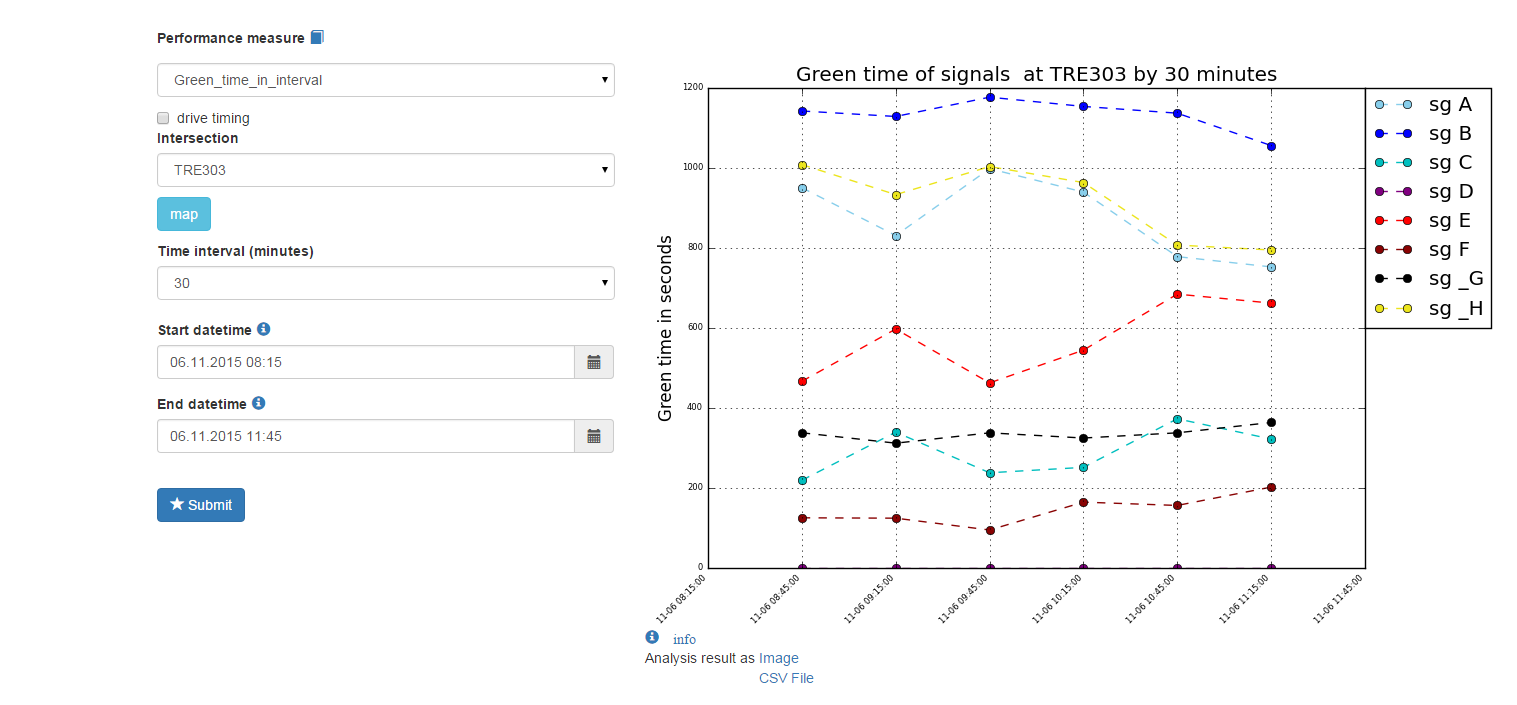
\includegraphics[width=1.0\linewidth]{interface.png}
	\caption{The user interface for analysis page of ImAnalysis}
	\label{fig:user interface}
\end{figure}

\section{Signal timing } \label{Signal timing}


\subsection{Green timing}

Green duration is the time duration of a external state ''green'' sequence from a signal group. Acquisition of green timing helps traffic engineers to check if signal timings are operated as designed and try to achieve the allocation of green to every direction is optimal. There are three measurements about green duration from different facets, that means every green phase could be recorded in seconds and percentile per cycle. In addition, the total green duration in specified time period is also available.

The following Figure ~\ref{fig:green timing} demonstrates the green duration in the intersection TRE303 from 14:00 to 14:40 on 10th, July, 2015.  The function calculates green duration per cycle. Multi curve lines represent all the signals at the selected intersection. As to each single line, the y-value of the solid point means the time duration of a green phase in seconds and x-value of points means the date and time when the green phase starts from. 

 During the selected time span, for the most time, signal group B takes up the longest green time, and the next are signal A and signal {\_}H with identical variety, as the map of the intersection TRE303 (figure ~\ref{fig:map of intersection TRE303}) shown, both signal A and pedestrian signal {\_}H control the direction from west towards east. Beside, the green timing of pedestrian signal {\_G} is almost fixed at 13 seconds.

\begin{figure}[!h]
	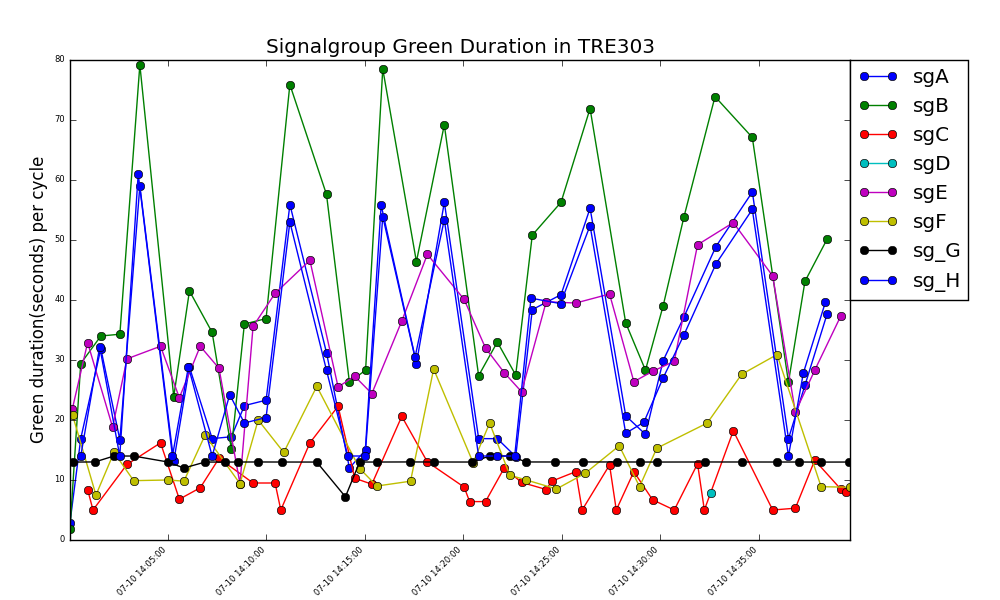
\includegraphics[width=\linewidth]{greenduration.png}
	\caption{Green timing}
	\label{fig:green timing}
\end{figure}

Figure ~\ref{fig:percentage of green} indicates the proportion of green time in the cycle time, which proves that the trend of percentage of green in the whole sequence of green, amber and red phases. The curve lines are not same with the green timing in seconds, but the rank of green percent for signals keeps in pace with their green timings. Only the signal B always occupied over 50{\%} percent.

\begin{figure}[!h]
	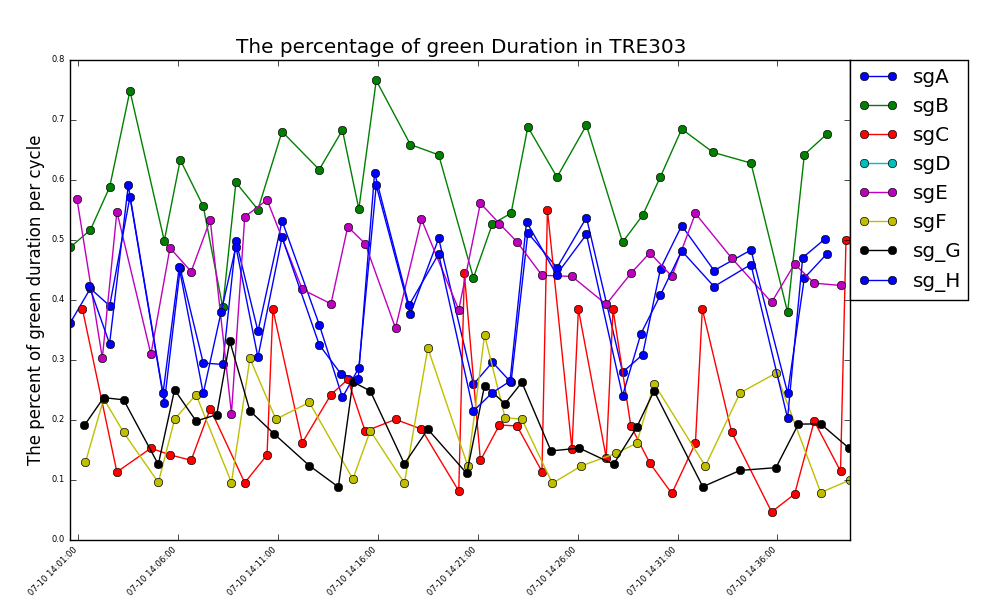
\includegraphics[width=\linewidth]{greenpercent.png}
	\caption{Percentage of green}
	\label{fig:percentage of green}
\end{figure}

Figure ~\ref{fig:map of intersection TRE303} Layout of the intersection TRE303 located at Satakunnakatu in city of Tampere, tells the locations of signals and loop detectors.  The movements controlled by signal A and signal B are critical movement, that is the reason that they occupied longer green times per cycle. 

\begin{figure}[!h]
	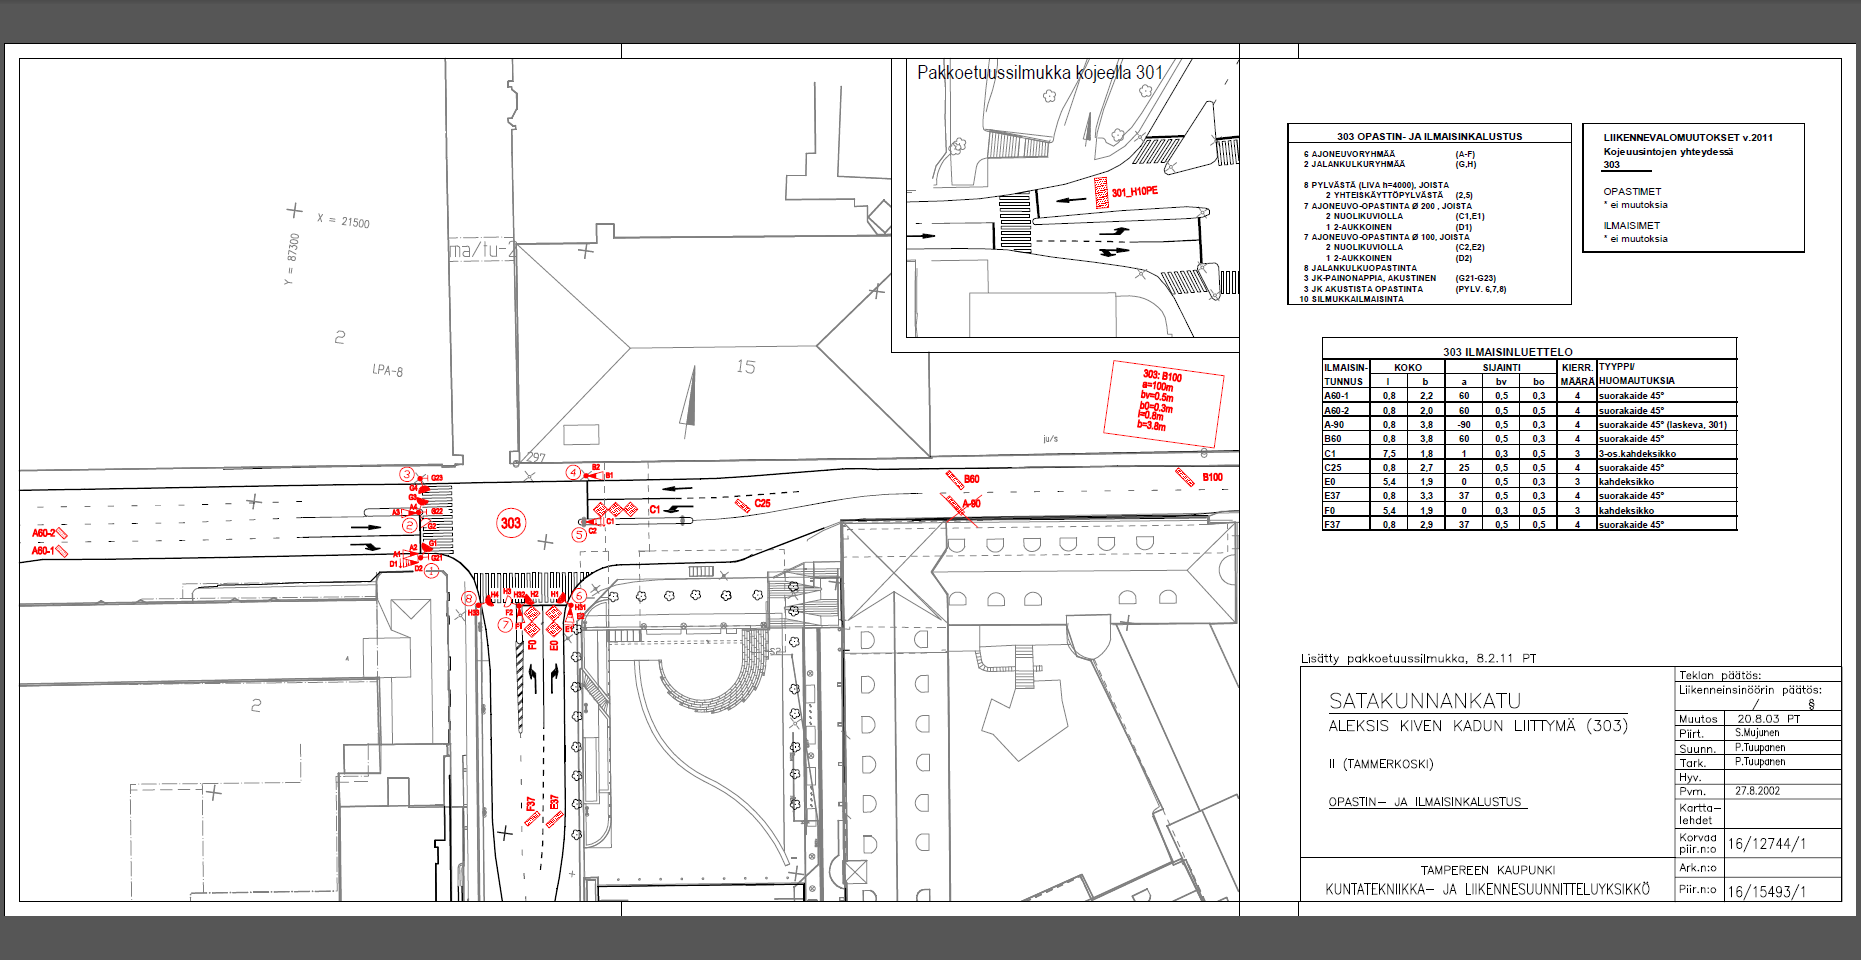
\includegraphics[width=\linewidth]{TRE303.png}
	\caption{Map of intersection TRE303}
	\label{fig:map of intersection TRE303}
\end{figure}

\subsection{Active green}

Active green is of importance to deduce efficiency of green timing. In general speaking, the more timing active green takes in the whole green phase, the more efficient it indicts. That is especially useful for those directions holding longer green time at intersections. In other words, if there is always considerable passive green existing on some way, traffic engineers might pay more attention to it and consider to enhance signal efficiency.

Based on the general knowledge, active green is the timing of a signal group from green start to the time when last vehicle comes. Oppositely, passive green is the timing after last vehicle comes until the end of green phase . However, from the internal state of signal group (''grint'') recorded by traffic signal controller, the time of state ''PASSIVE{\_}GREEN'' is counted, while the active green timing is left green excluding ''PASSIVE{\_}GREEN'' during a green sequence.  Hence, the calculation of active and passive green based on the two principles separately is implemented and compared.

The function calculates active green length per cycle of the selected signal, comparing its timing of passive green based on the two different definitions. This stacked bar chart shows proportion of both active green and passive green. The x-axis is actual time of a day, and y axis is time duration in seconds. 

\begin{figure}[!h]
	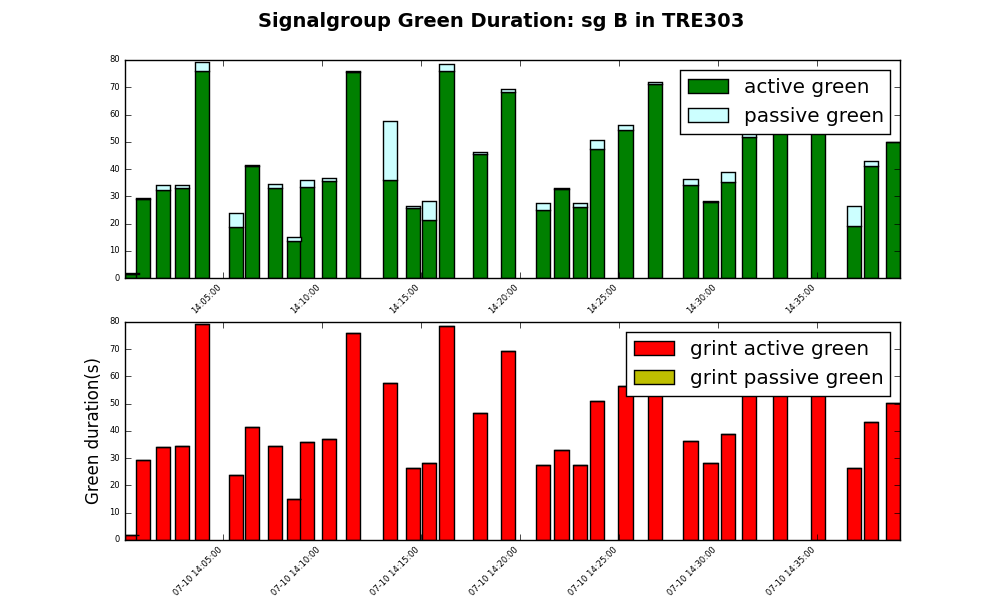
\includegraphics[width=\linewidth]{activegreen.png}
	\caption{Active green}
	\label{fig:active green}
\end{figure}

The Figure ~\ref{fig:active green} shows the result of this measure for signal group B at intersection TRE303 in Tampere from 14:00 to 14:40 on 10th, July, 2015. 

The upper chart is visualized based on occupancy of the detector, every bar represents length of an entire green sequence. During ''active green'' (dark green), there are requests for vehicles received by any associated detector. Conversely, during ''passive green'' (light blue), it starts at the moment that last vehicles came and no detector is occupied at all, and ends this green phase. Signal B as the signal group which operates the longest green time in the intersection, little green is squandered when no vehicle is detected, though it could be absolutely active under ideal condition. 

The second chart shows the proportion of active and passive green based on ''grint'' state codes, the red part means 'grint' active green timing. And the yellow part is for the time duration when the signal state is ''PASSIVE{\_}GREEN''. By comparison, the distribution of active green and passive green times are not corresponding with the upper bar chart. In the specified time span, there is no ''PASSIVE{\_}GREEN'' at all. 


\section{Queue and delay at intersections}

\subsection{Queue length}

\begin{figure}
	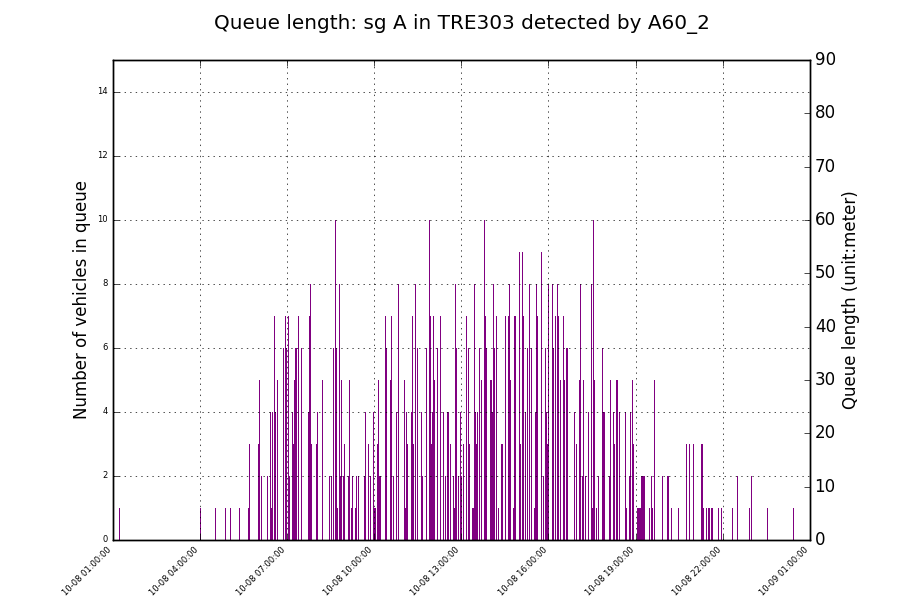
\includegraphics[width=\linewidth]{queuelength.png}
	\caption{Queue}
	\label{fig:queue}
\end{figure}

\begin{figure}[!h]
	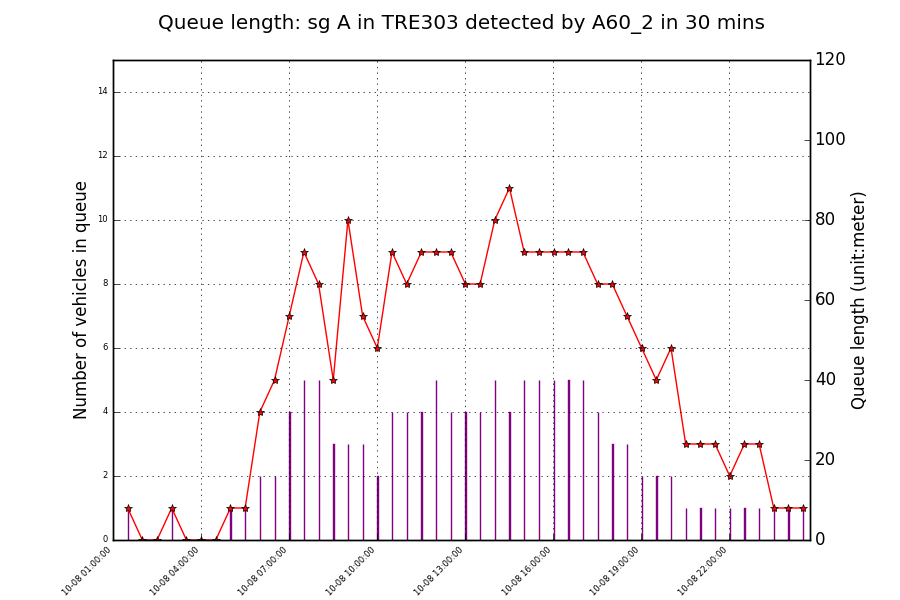
\includegraphics[width=\linewidth]{queue2.png}
	\caption{Average and maximum queue in every 30 minutes}
	\label{fig:average and maximum queue in every 30 minutes}
\end{figure}

At signalized intersections, queue length is the queue of vehicles at the end of red time (red-end) by lanes according to detectors.  Queue length estimation is a pretty important intersection performance measurement. Efficient offset times should consider the time to discharge the queue at intersections, moreover, estimation of queue in next cycle is good for optimizing the entire signal system. 

Traffic engineers can use queue analysis to identify problems and improve the efficiency of traffic signal control by maximizing traffic throughput at an intersection. Furthermore, calculation of queue could assist decision makers enhance the service from individual intersection to entire traffic network.

This measurement calculates length of stationary queue in meters and amount of vehicles forming a queue on the end of red time. The plot of this measurement has dual y-axis. The left y-axis is number of vehicles and right y-axis is length of queue in meters, while x-axis is actual time when red phase ends.  

The figure ~\ref{fig:queue} shows the result of queue length estimation via detector A60{\_}2 under controlling of signal group A at intersection TRE303 in Tampere from 00:00 to 23:59 on Thursday, 8th, October, 2015. From midnight to 5:00, almost no vehicles went through and at about 6:00 in the morning, queues start to occur. The figure ~\ref{fig:average and maximum queue in every 30 minutes} illustrates average and maximum value of queue in every intervals. The red curve line with asterisk symbol over the bars is combined by maximum queues and the bars are average queue in every half an hour. 



\subsection{Waiting time at intersections}


Waiting time estimates the extra time vehicles in queues spend at intersections before moving from stop bar.Delay at an intersection also can be approximately treated as waiting time that a vehicle spends at the intersection comparing the time it should pass without any hindrance.  The approach to calculate waiting time is related to queue length and headway of vehicles at intersections. The default value of headway is 2 second and distance between two successive vehicles as they pass a point on the roadway is 8 meters. 

%%%%%%% Multiple images
\begin{figure}[ht!]
	\begin{center}
		%
		\subfigure[Waiting time in time interval]{%
			\label{fig: waiting time in time interval}
			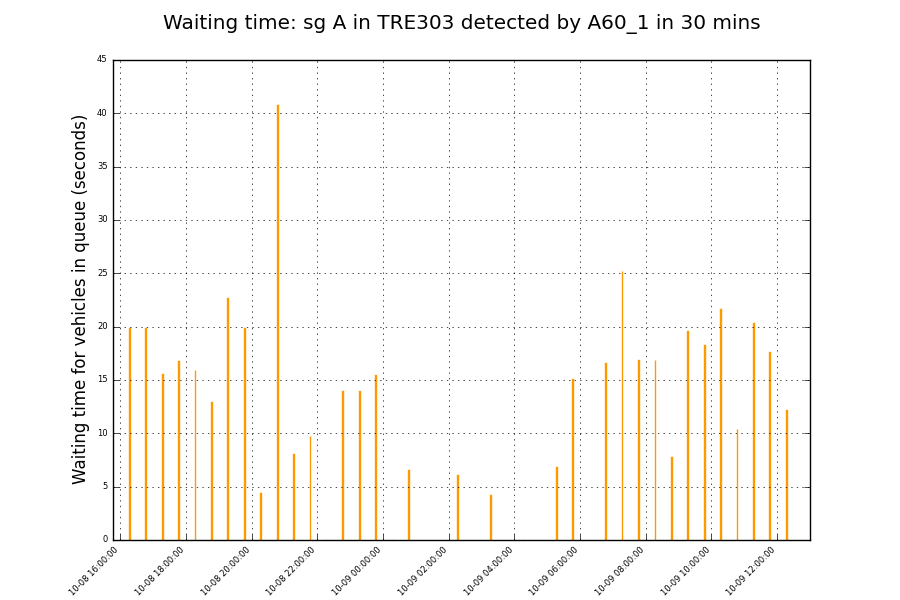
\includegraphics[height=5cm,width=0.5\linewidth]{waitingtimeininterval.png}
		}%
		\subfigure[Waiting time]{%
			\label{fig: waiting time}
			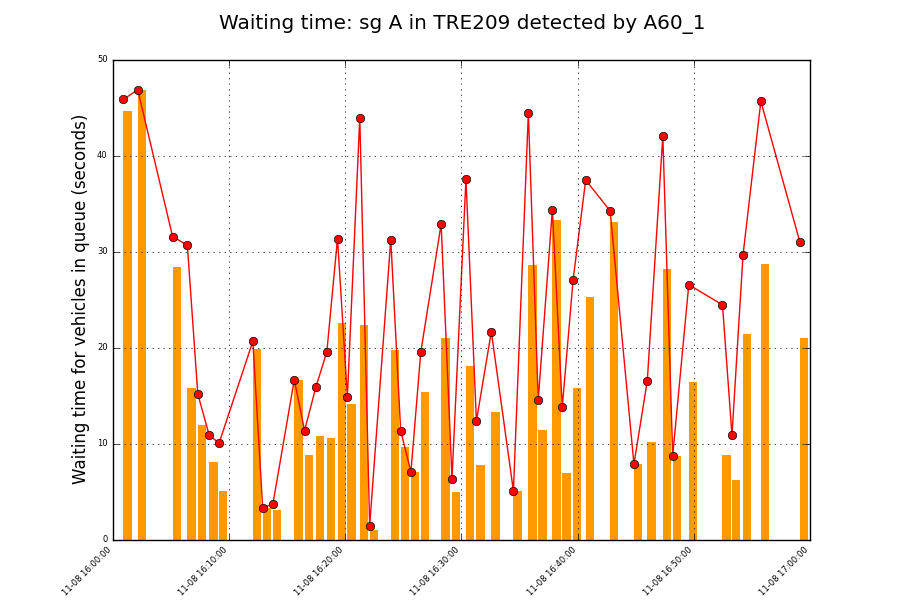
\includegraphics[height=5cm, width=0.5\linewidth]{waitingtime.png}
		}\\ %  ------- End of the first row ----------------------%
	\end{center}
	\caption{%
		Waiting time
	}%
	\label{fig: waiting time}
\end{figure}


The figure \ref{fig: waiting time} shows waiting time of vehicles at intersection TRE303 detected by detector A60{\_}1. The subfigure \ref{fig: waiting time in time interval} represents the estimation waiting time in average for every queued vehicle in every 30 minutes from 18:00, 8th of October to next day 13:00. The subfigure \ref{fig: waiting time} calculates waiting time of vehicles in every queue. An orange bar is mean of waiting time in this queue and a red dot is the maximum waiting time.

\section{Traffic capacity}


\subsection{Saturation flow rate}

Saturation flow rate is an elemental parameter to measure the traffic capacity and vehicle discharging time at intersections [~\cite{Shao:2012}]. The saturation flow rate crossing a signalized stop line is defined as the number of vehicles per hour that are able to cross the line if the signal remained green all of the time. Naturally, certain traffic and roadway condition influences saturation flow rate. For example, if the approach is a narrow lane, the traffic have to keep a longer gap; if there are large numbers of turning movements and heavy vehicles, the saturation flow rate reduces as well.

Since the saturation flow rate depends on roadway and traffic condition, it is a complicate matter to calculate it, which can vary substantially from one region to another. ImFlow uses the pre-defined saturation flow rate in different time and areas. However, the external condition might be not unchanged all the time, so there is a function to estimate the saturation flow rate by real data. However, the movements of vehicles in reality cannot fully simulate  the idealized condition, hence, the result of this function will be reasonably lower than the actual value.

The function estimates saturation flow rate for each lane controlled by the selected signal group at intersections using real data following the equation ~\ref{eq:saturation flow rate}, assuming that every vehicle in the queue from first m-to-n is in a stable moving platoon.



\begin{equation} \label{eq:saturation flow rate}
\overline{s}=\frac{1}{N}\sum_k^NT\frac{m-n}{T_{m}-T_{n}}
\end{equation}

Where, $\overline{s}$ is the average value of saturation flow, $N$ is the number of vehicles flows which satisfying the condition, T is unit time( one hour) in seconds, $T_{m}$ and $T_{n}$ are the time when the m-th and n-th vehicles passing through. Taking advantage of the suggestion from \cite{HCM:2010}, m equals 10 and n is 4 in the traffic queue. Using the approach, average value of observed discharge headway is known.

The algorithm requires real data to satisfy a high restrict that traffic is as dense as possible reasonably to pass the intersection in a long traffic flow. Hence, according to some selections, the result returns null because no data satisfy the calculation conditions. As to the plot, x-ticks are the names of detectors associated to the specified signal group, y-axis shows the number of vehicle. 

\begin{figure}[!h]
	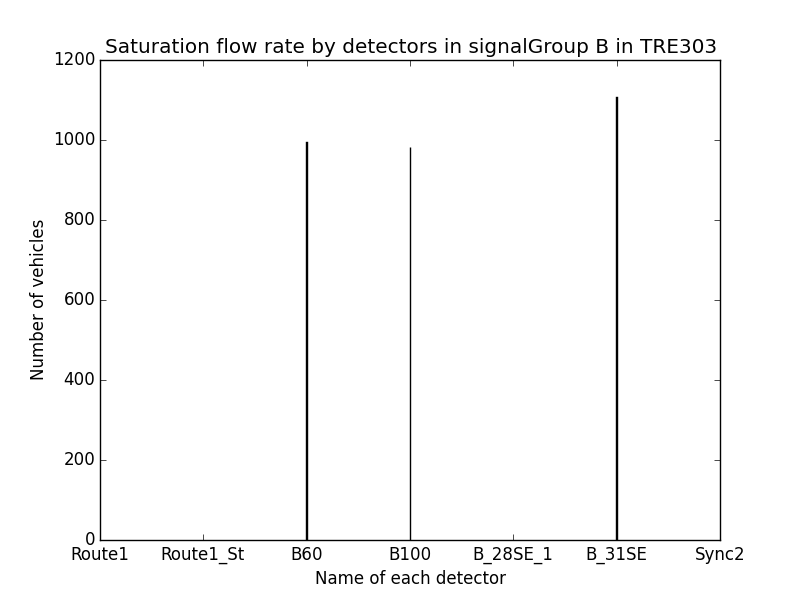
\includegraphics[width=\linewidth]{saturationflowrate.png}
	\caption{Saturation flow rate for sg B at TRE303}
	\label{fig:saturaionflowrate}
\end{figure}

The figure ~\ref{fig:saturaionflowrate} illustrates saturation flow rate for lanes associated with signal group B at intersection TRE303 in Tampere on 4th, October, 2015. As the image showing, the estimated saturation flow rates at the place of detector B60, B100 and B{\_}31SE are available. Since B60 and B100 are located at the same lane, it is reasonable that their values, 996 vphgpl and 983 vphgpl are so close, whereas saturation flow rate at detector B{\_}31SE is 1107 vphgpl. 


\subsection{Maximum capacity}

Capacity is an adjustment of the saturation flow rate with the real signal green time, as most signals are not allowed to keep an hour continuous green for a certain movement, except the ''sleep mode'' of major road signals permitting long time green during the midnight in Finland, if no vehicle requests from minor roads. For instance, if one approach has half an hour green in total per hour, the capacity can be deduced to half of the saturation flow rate in one hour time interval. 

Maximum capacity is defined as the maximum number of vehicles can be reasonably expected to traverse a point or a uniform segment of a lane or roadway during a given time period under prevailing roadway, traffic control conditions. The formula to calculate maximum capacity is given in equation ~\ref{eq:capacity}:

\begin{equation} \label{eq:capacity}
c = (g\div C)\times s
\end{equation}

where $c$ represents capacity, $g$ is the effective green time for the phase in seconds, $C$ is cycle length in seconds and $s$ is saturation flow rate. 

Based on your requirements, capacity can be calculated on different levels, either for each separate lane or lump the lanes in a direction together. In this application, the calculation of capacity is for signal lane by a selected detector in customized time period. What worthy mentioning is, to ensure that critical lane volumes are adequately served, the capacity of that lane should be checked in the same time interval.

It  calculates the total number of vehicles could pass over the specified detector during the sum of green timing in a certain time period (5 minutes, 10 minutes and 1 hour etc.).  Maximum capacity is positive correlated with saturation flow rate on a lane and green time in a period of a signal group. As to the plot on this measure, the x-coordination of the green solid diamonds is actual starting time of every time interval, and its y-coordination indicates the number of vehicles. The dashed line passes through all diamonds by time to show the trend of maximum capacity.  

\begin{figure}[!h]
	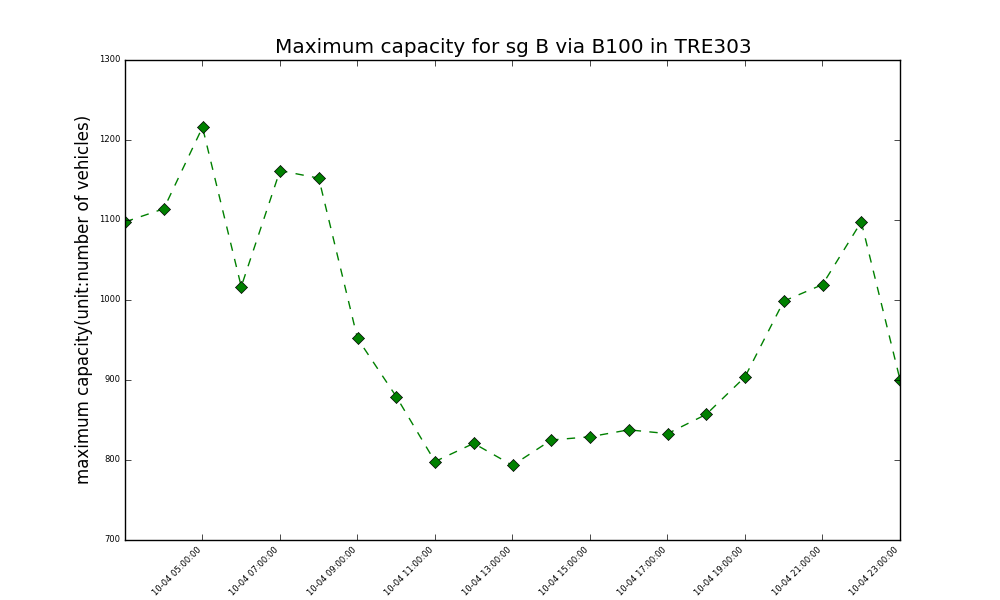
\includegraphics[width=\linewidth]{maximumcapacity.png}
	\caption{Maximum capacity}
	\label{fg:maximumcapacity}
\end{figure}

The figure~\ref{fg:maximumcapacity} shows maximum capacity of the lane where detector B100 located in one-hour interval at the intersection TRE303 at Tampere during the whole day on 4th, October. Due to signal B controls the major approach, the maximum capacity keeps high value over 1000 from midnight to 7:00 am in the morning.

\section{Volume}

Traffic volume is the procedure to determine mainly the volume of traffic moving on the roads at a particular point or a uniform segment during a particular time period. Volume of a day or an hour can vary vastly, depending on different days of the week and how busy time of the day is. 

Basically, there are two techniques of volume counting at intersections: volumes per detector and volumes per link. In the research, only the former one is used.

This measurement counts that the total number of vehicles could pass over the specified detector on a lane during certain time period (5 minutes, 10 minutes and 1 hour etc.). Two functions support this traffic performance measurement: ''Volume on a single direction'' and ''Volumes by customized multiple directions/detectors''. 

\begin{figure}[h!]
	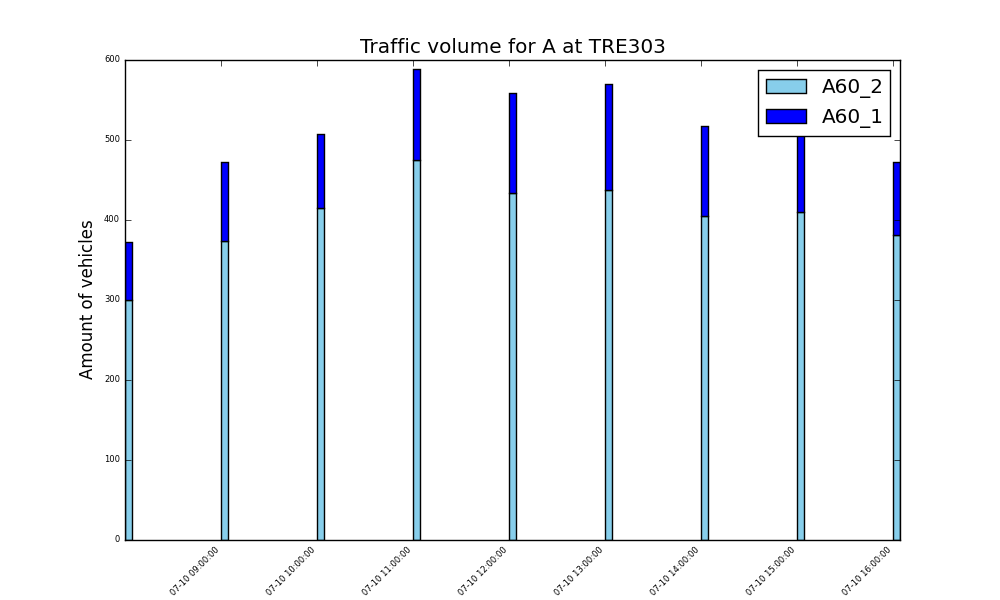
\includegraphics[width=\linewidth]{volume.png}
	\caption{Volume on a direction }
	\label{fg:volume on a direction}
\end{figure}

\begin{figure}[h!]
	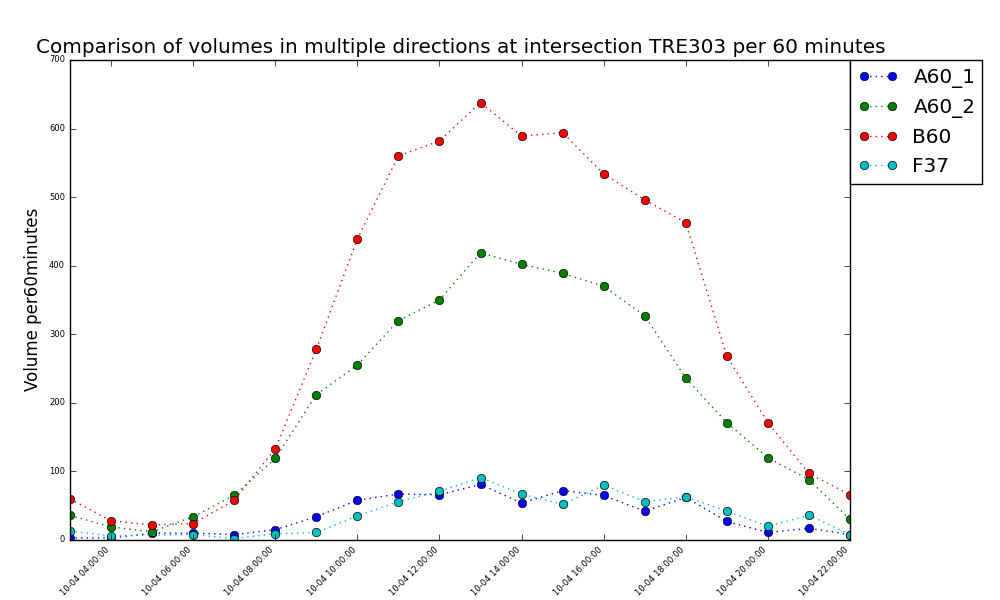
\includegraphics[width=\linewidth]{volumes.png}
	\caption{Volume on multiple directions }
	\label{fg:volume on multiple directions}
\end{figure}

\begin{itemize}
	\item Volume on a direction
\end{itemize}


Select a loop detector for counting vehicles, if there are more than one lanes paralleling with the selected one on a same direction,  the volumes of all the grouped lanes will be calculated and shown as parts of the stacked bars over times like the figure ~\ref{fg:volume on a direction}. The x-coordination of bars is the starting time of intervals and y-axis indicates traffic volume.

 Figure ~\ref{fg:volume on a direction} illustrates the volume on the two lanes controlled by signal group A at the intersection TRE303 on 10th, July from 8:00 am to 17:00 pm in 1-hour interval. The highest volume at that place during that day is from 11:00 am to 12:00 pm with 590 vehicles discharging by the two lanes. This straight lane which is equipped with the detector A60{\_}2 is much busier than the right-turning lane with the detector A60{\_}1 and the result is recorded in table ~\ref{Table of volumes at the lanes of signal A at TRE303} .  

\begin{table}[h!]
	\centering
\begin{tabular}{ |p{3cm}||p{3cm}|p{3cm}|  }
	\hline
	\multicolumn{3}{|c|}{VOLUME} \\
	\hline
	Time     & A60{\_}1 &  A60{\_}2\\
	\hline
	2015-07-10 09:00   & 73    &300 \\
	2015-07-10 10:00 &   99 & 374\\
	2015-07-10 11:00 &93 &415 \\
	2015-07-10 12:00 &114 & 475 \\
	2015-07-10 13:00 & 125 & 434\\
	2015-07-10 14:00 & 132  & 434\\
	2015-07-10 15:00 & 113  & 438\\
	2015-07-10 16:00 & 107  & 410\\
	\hline
\end{tabular}
\caption{Table of volumes at the lanes of signal A at TRE303}
\label{Table of volumes at the lanes of signal A at TRE303}
\end{table}



\begin{itemize}
	\item Volumes by customized multiple directions/detectors
\end{itemize}

On the other hand, selecting more than one detectors and comparing the volume flows on multiple directions is allowable for observing and predicting traffic volumes coming from different directions.


The figure ~\ref{fg:volume on multiple directions} demonstrates the visualized results that volumes counting in every hour at the spots of detector A60{\_}1, A60{\_}2, B60, F37 on the lanes which equipped them separately in a day, which gives intuitive comparison of traffic volumes at this intersection TRE303 and is helpful to determine the critical roads and the minor roads, design and adjust the traffic signal timings. 

\section{Arrival on green}
\subsection{Arrival on green percentage}

Arrival during green is defined as vehicles in movements arriving at intersection stop bar during green phases and can be calculated as the equation ~\ref{eq:arrival on green}:

\begin{equation} \label{eq:arrival on green}
P = \frac{N_{g}}{(N_{g})+(N_{r})}
\end{equation}

where arrival on green is noted as $P$, $N_{g} $ is the number of vehicles arriving during green time and $N_{r}$ is the number of vehicles arriving during red time.

\begin{figure}[h!]
	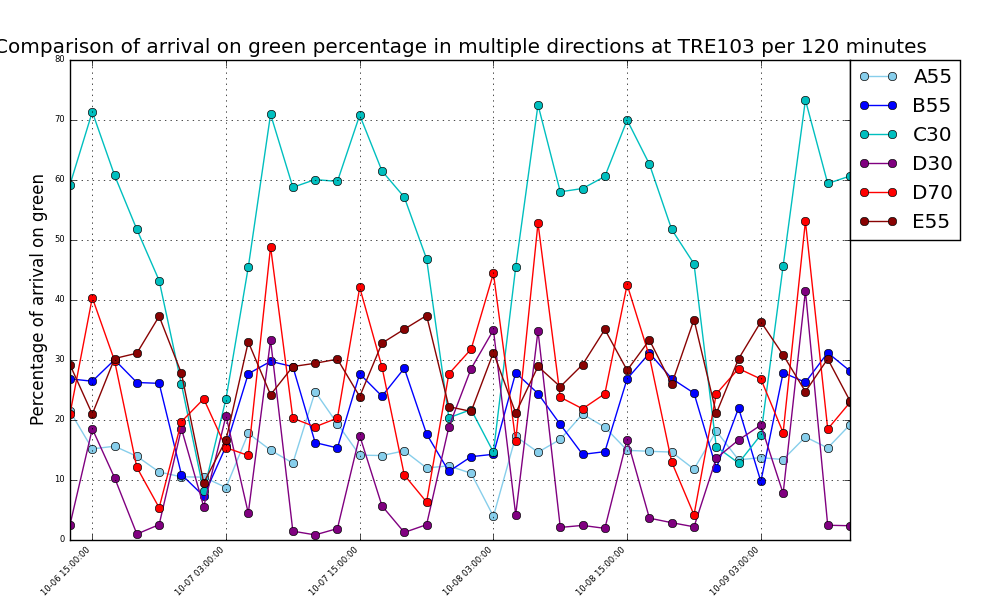
\includegraphics[width=\linewidth]{arrivalongreenpercent.png}
	\caption{Percentage of arrival on green }
	\label{fig:percent of arrival on green}
\end{figure}

The traffic number is counted by specified detectors in a time period (5 minutes, 10 minutes and 1 hour etc.). It is a useful traffic performance to evaluate the signal timing performance at individual intersections and deduce the density of traffic flow. Usually, the high percentage of arrival on green is an indicator of smooth traffic. 

Figure ~\ref{fig:percent of arrival on green} depicts the situation of arrival during green in three days from 12:00, 6th to 12:00 by 2-hour interval, 9th of October at TRE103, one of the busiest intersections located nearby Tampere railway station. It can be seen from the figure that arrival on green in a single direction is roughly repetitive over times. 

Take the volume calculated using C30 as an instance, in every day, the two peak values of arrival during green reaching 70\% occur in the same periods:8:00 am to 10:00 and 16:00 to 18:00 while during the quite time of every day between midnight 12:00 am to 6:00 am, the value remains lower than 30\%. It implies that the controlling of signal timing is pretty effective to this lane holding largest volume in day time.

Similar trend occurs on the directions where D30 and D70 are. As for the situation on the other three detectors A55, B55 and E55, they are more fluctuated in a smaller range, but the overall trend conforms that during day time, the percentage that vehicles arriving at this intersection is higher.



\subsection{Arrival on green ratio}

\begin{figure}[h!]
	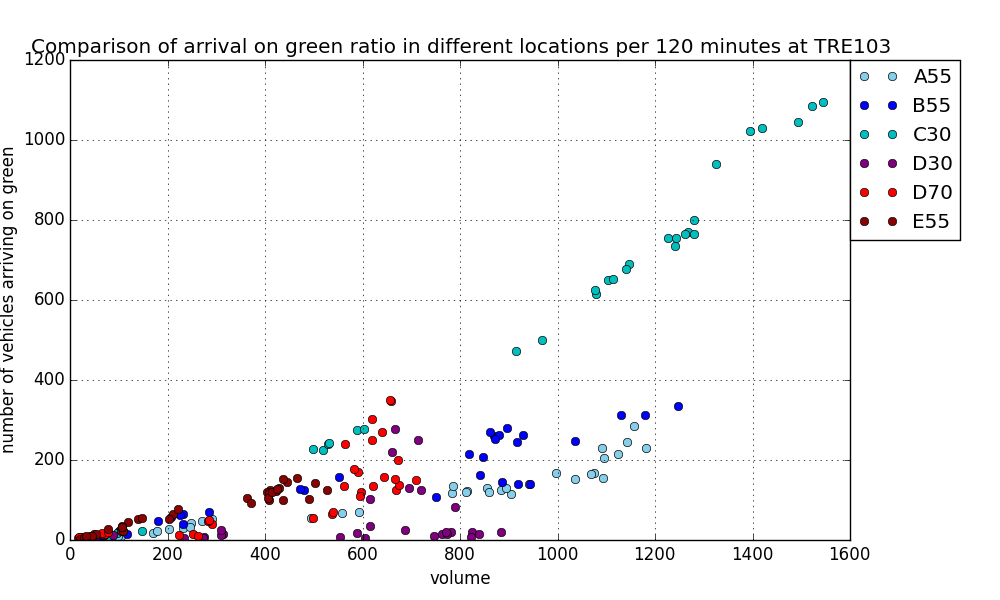
\includegraphics[width=\linewidth]{arrivalongreenratio.png}
	\caption{Ratio of number of arrival on green and volume }
	\label{fig:ratio of number of arrival on green and volume}
\end{figure}

\begin{figure}[h!]
	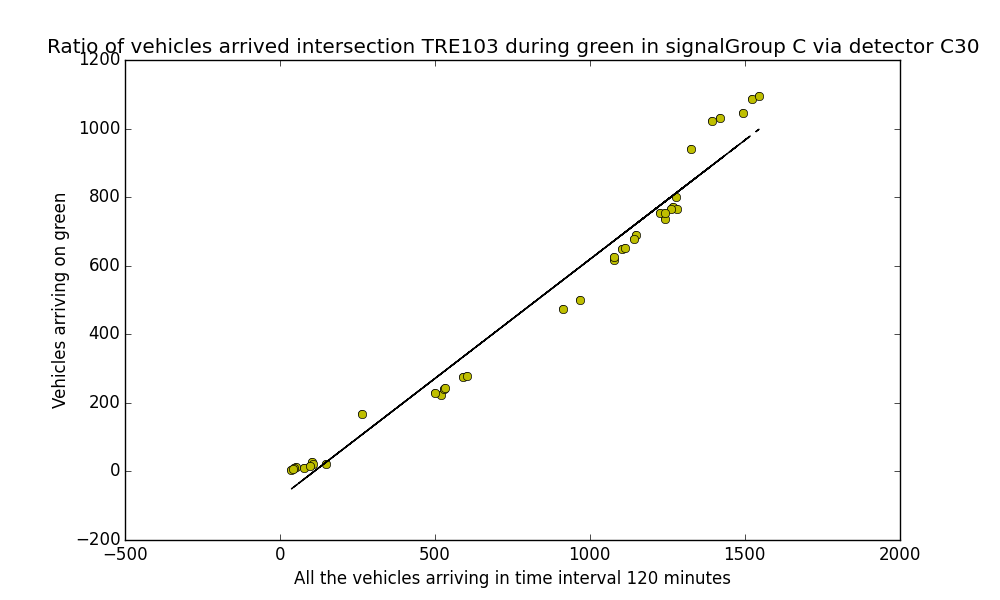
\includegraphics[width=\linewidth]{oneratio.png}
	\caption{Ratio of arrival on green by C33 at TRE103 with linear regression}
	\label{fig:ratio of arrival on green by C33 at TRE103}
\end{figure}

Arrival during green is defined as vehicles arriving at intersection stop bar during green time. The ratio is another measurement from different dimensions related to arrival during green to reveal the issue. 

The ratio of arrival during green is used to mine the relation between volume and arrival on green performance. As is shown by the figure ~\ref{fig:ratio of number of arrival on green and volume}, it compares the scalar variable, the number of vehicles arriving during green with the total volume under the same prerequisite with the figure ~\ref{fig:percent of arrival on green}. 

Those scatter points are clustered by their colors representing the detectors. The most outstanding cluster are from detector C30 with both higher total volume and number of arrival during green. When taking more than 600 total volume, it has much more vehicles arriving during green time than others. Comparatively,the direction of detector E55 holds least vehicles, D30 has the lowest value of arrival on green, A55 and B55 are in the middle class. 

The figure ~\ref{fig:ratio of arrival on green by C33 at TRE103} specifically depicts this performance for detector C30. The linear regression is for modelling the relationship between volume and number of arrival on green. The slope of the regression line is 0.6, which means the average percentage of arrival on green at detector C30 is 60\%, whereas the slopes for A55, B55, D70 are 0.15, 0.25 and 0.25 respectively.



%%%%%%%%%%%%%%%%%%%%%%%%%%%%%%%%%%%%%%%%%%%%%%%%%%%%%%%%%%%%%%%%%%%%%
\chapter{Validation and analysis  }\label{ch:Validation of evaluation}

Performance qualification is very important to verify accuracy of measurements and efficiency of algorithms. Comparison with traffic performance reports created by ImFlow on some level to verify and evaluate efficiency of those models is a critical approach in this chapter. Three measurements are compared with results on ImFlow, including green duration, traffic volume and saturation flow rate. As for others measurements, they will be researched according to case studies and specific investigations.  

\section{Validation of results}
\subsection{Comparison on green duration}

In the previous chapter (\nameref{ch:The analysis and visualization}) , measurements of signal green timing are introduced in some aspects. Besides the two mentioned measurements: green duration in seconds per phase and the percentage of green duration per phase,  the cumulative value of green timing in a specified period is also a good measurements of traffic performance, which is also provided by ImFlow.

Therefore, in order to verify the accuracy of measurements for green timing, we will take advantage of this same traffic performance measured by ImFlow. 


%%%%%%% Multiple images
\begin{figure}[ht!]
	\begin{center}
		%
		\subfigure[green time on ImFlow]{%
			\label{fig:green time on ImFlow}
			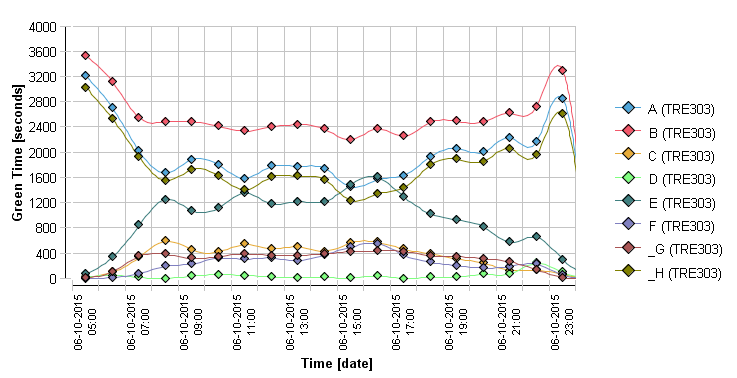
\includegraphics[height=5cm, width=.5\linewidth]{imflowgreentime.png} 
		}%
		\subfigure[green time]{%
			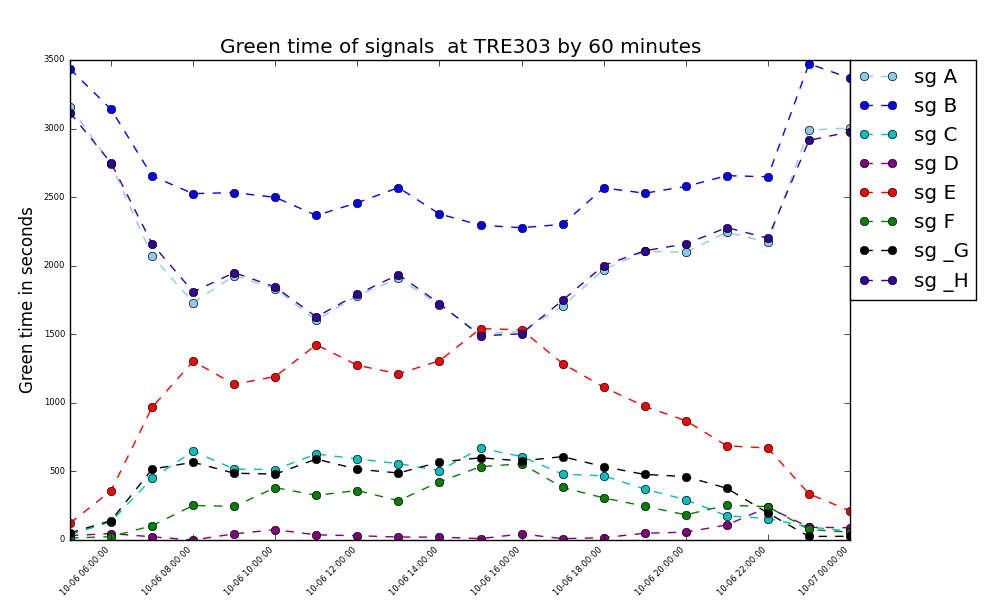
\includegraphics[height=5cm, width=.4\linewidth]{imanalystgreentime.png} 
			\label{fig:green time on ImAnalyst} 
		}\\ %  ------- End of the first row ----------------------%
	\end{center}
	\caption{%
		Comparison for green timing calculated by two sources
	}%
	\label{fig: comparison of the reports of green time from ImFlow and ImAnalyst}
\end{figure}
%%%%%%% 

\begin{figure}[h!]
	\centering
	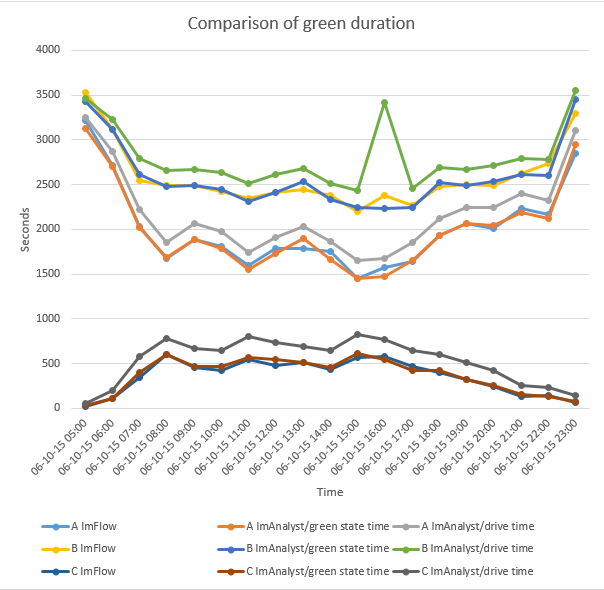
\includegraphics[width=\linewidth]{mergegreen.png}
	\label{fig:comparison of green duration calculated by two sources}
	\caption{comparison of green duration calculated by two sources}  
\end{figure}

\begin{table}[h!]
	\begin{tabular}{ |p{3cm}||p{1.5cm}|p{2cm}| p{2cm}|p{2cm}|p{1.5cm}| }
		\hline
		\multicolumn{6}{|c|}{Green timing in seconds for signal A} \\
		\hline
		Start time     & ImFlow & Analysis tool & time difference & Overlapping (\%)&green percents(\%) \\
		\hline
		2015-10-06 05:00   & 3214    &3131.889 & +72.111 & 102.6 & 89\\
		2015-10-06 06:00 &   2709 & 2699.616 & +9.384 & 100.37 & 75\\
		2015-10-06 07:00 & 2031 &2022.785 & +8.215 & 100.4 &56 \\
		2015-10-06 08:00 & 1677 & 1687.098 & -10.098 & 99.4 & 46 \\
		2015-10-06 09:00 & 1888 & 1882.449 & +5.001 &100.3 &52\\
		2015-10-06 10:00 & 1805  & 1787.639 &  +17.361 & 101 &50\\
		2015-07-10 11:00 & 1591 & 1557.597 &+33.403 & 102.2 & 44\\
		2015-07-10 12:00 & 1782  & 1736.25 &  +45.75 &  102.56 &49\\
		2015-07-10 13:00 & 1781  & 1869.110 & -77.110 & 95.3 & 49 \\
		2015-07-10 14:00 & 1794  & 1666.384 & +127.616 & 107.68 &48\\
		2015-07-10 15:00 & 1455  & 1452.086 &+2.914 & 100.2 & 40\\
		2015-07-10 16:00 & 1577 & 1474.004 & +102.996 & 106.98 &43\\
		\hline
	\end{tabular}
	\caption{Comparison the green tming calculated by the two sources}
	\label{tb: comparison the green tming calculated by the two sources}
\end{table} 

Figure ~\ref{fig: comparison of the reports of green time from ImFlow and ImAnalyst} demonstrates the two original plots for the cumulative green time in seconds from 5:00 to 24:00 on 6th, October, 2015 at the intersection TRE303 in 1 hour interval. The upper plot is created by ImFlow, one of the released productions by Imtech traffic. And the bottom plot is the result rendered by the traffic signal analysis tool. 

With comparison of the two plots, the trend of two curve lines representing the green duration are consistent. It proves that the calculation of green timing by the application is reasonable and able to stimulate the real signal timing on certain level, while the slight difference of values between the two plots still exists. Thus, the table ~\ref{tb: comparison the green tming calculated by the two sources} extracts signal group A in the time range of 05:00 and 16:00 of that day, as an instance to compare the values calculated by the analysis tool and ImFlow on details.

One row in the table ~\ref{tb: comparison the green tming calculated by the two sources} describes that in one-hour time period with the start time specified in first column, the pair of green timings are recorded by the two sources separately. The time difference between the two values is calculated and the percentage of overlapping converges to 100{\%}, and the largest deviation is 7.68\% happened during 14:00  to 15:00. 


\subsection{Comparison on volume}


\begin{figure}
	\hspace*{-.5in}
	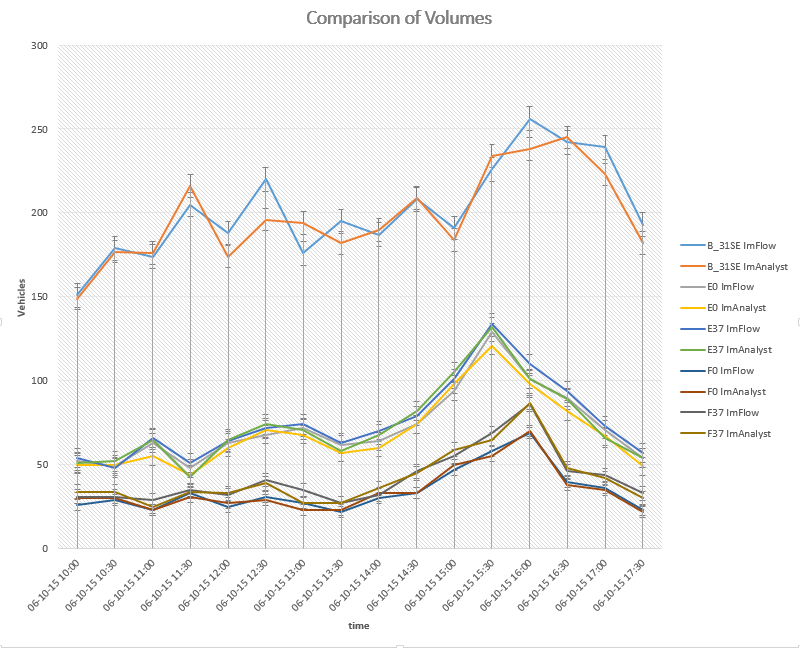
\includegraphics[width=1.2\linewidth]{mergevolumes.png}
	\caption{Comparison of Volumes calculated by the two systems}
	\label{fig:Book1(Recovered)}
\end{figure}

\begin{table}
\begin{tabular}{ |p{3cm}||p{.8cm}|p{.8cm}| p{.8cm}|p{.8cm}|p{.8cm}|p{.8cm}|p{.8cm}|p{.8cm}|p{.8cm}|p{.8cm}| }
	\hline
	\multicolumn{11}{|c|}{Volume at TRE303} \\
	\hline
	{time}  & \multicolumn{2}{|c|}{B\_31SE} & \multicolumn{2}{|c|}{E0}  & \multicolumn{2}{|c|}{E37}& \multicolumn{2}{|c|}{F0} & \multicolumn{2}{|c|}{F37}   \\ \hline
	& (a) & (b) & (a) & (b) & (a) & (b) & (a) & (b) & (a) & (b) \\ \hline
	06-10-15 10:00 & 151 & 149 & 52 & 50 & 54 & 51 & 26 & 30 & 31 & 34 \\ \hline
	06-10-15 10:30 & 179 & 177 & 49 & 50 & 48 & 52 & 29 & 30 & 31 & 34 \\ \hline
	06-10-15 11:00 & 174 & 176 & 63 & 55 & 66 & 65 & 23 & 23 & 29 & 25 \\ \hline
	06-10-15 11:30 & 205 & 216 & 48 & 44 & 51 & 43 & 33 & 31 & 35 & 34 \\ \hline
	06-10-15 12:00 & 188 & 174 & 63 & 60 & 64 & 65 & 25 & 27 & 32 & 33 \\ \hline
	06-10-15 12:30 & 220 & 196 & 68 & 71 & 72 & 74 & 31 & 29 & 41 & 39 \\ \hline
	06-10-15 13:00 & 176 & 194 & 72 & 68 & 74 & 71 & 27 & 23 & 35 & 27 \\ \hline
	06-10-15 13:30 & 195 & 182 & 62 & 57 & 63 & 58 & 22 & 23 & 27 & 27 \\ \hline
	06-10-15 14:00 & 187 & 190 & 64 & 60 & 70 & 68 & 30 & 33 & 32 & 36 \\ \hline
	06-10-15 14:30 & 208 & 209 & 74 & 74 & 79 & 82 & 33 & 33 & 46 & 45 \\ \hline
	06-10-15 15:00 & 191 & 184 & 94 & 98 & 101 & 105 & 47 & 50 & 55 & 59 \\ \hline
	06-10-15 15:30 & 226 & 234 & 129 & 121 & 134 & 132 & 58 & 55 & 69 & 65 \\ \hline
	06-10-15 16:00 & 256 & 238 & 101 & 98 & 110 & 101 & 69 & 70 & 86 & 87 \\ \hline
	06-10-15 16:30 & 242 & 245 & 90 & 82 & 94 & 89 & 40 & 38 & 46 & 48 \\ \hline
	06-10-15 17:00 & 239 & 223 & 71 & 67 & 73 & 66 & 36 & 35 & 44 & 42 \\ \hline
	06-10-15 17:30 & 193 & 182 & 54 & 49 & 57 & 54 & 23 & 22 & 33 & 30 \\ \hline
	total & 3230 & 3169 & 1154 & 1104 & 1210 & 1176 & 552 & 552 & 672 & 665 \\ \hline
	average diff & \multicolumn{2}{|c|}{4.07} & \multicolumn{2}{|c|}{3.33} & \multicolumn{2}{|c|}{2.27}  &  \multicolumn{2}{|c|}{0} & \multicolumn{2}{|c|}{0.47}  \\ \hline
\end{tabular}
	\caption{Comparisone volumes calculated by two sources}
	\label{Comparison volumes with Imflow}
\end{table}

Traffic volume counting per loop detector is another significant indicator of intersection traffic provided by both ImFlow and ImAnalyst.  

The original plots from the two system under same limitation of time span and all other parameters are merged in the figure ~\ref{fig:Book1(Recovered)}, which demonstrates the volumes detected by five ImFlow-recommended detectors from 10:00 to 18:00 at intersection TRE303 by 30-minutes time interval. Among the detectors,E0 and E37 that are associated with signal E and detectors serving signal F are on the lanes side by side, signal E is right-turning(south-towards-west) and another one is left-turning(south-towards-east). From the graph it is clear that the volumes counted by the detectors on a lane are almost overlapping completely no matter ImFlow or ImAnalyst is used.

Figure ~\ref{fig:Book1(Recovered)} presents the result with error bars in both positive and negative directions. It is easily observed the fine distinct between the plots with a table of precise data under the graph.  Error bars are a graphical representation of variability of data, and are used to indicate the error or uncertainty in a measurement. They gives a general range of how precise the measurement is. Usually, error bars stand for the standard deviation of uncertainty or standard error or confidence interval. Most error bars for the paired data overlap, the conclusion is that the difference between the mean value of them is not statistically significant.

 It is obvious that volumes per detector B\_31SE have largest difference and sometime even their error bars are isolated. However, the average difference of paired volumes is only 4 vehicles.

\subsection{Comparison on saturation flow rate}

The approach of calculating saturation flow rate on ImAnalyst is to estimate the value using live data. The advantage of this function is reflecting the actual traffic saturation flow rate considering the roadway condition and other environment factors. The drawback of this approach is that easily lead to underestimation using live data to simulate idea data. 

The following image ~\ref{fig:Saturation flow rate} is saturation flow rate for signal B at TRE303 on 6th, Nov, 2015. The estimation calculated via B60, B100, B{\_}31SE is 1224, 1274, 1130 in terms of passenger car units(pcu) separately. However, saturation flow rate for signal B on ImFlow is always 1800 as the figure ~\ref{fig:Saturation flow rate provided by ImFlow}. It is quite common to assume an ideal saturation flow rate and adjust it for prevailing conditions using adjustment factors like ImFlow does. The study provides a new aspect to verify and test the value for a specific case using live data without any adjustment for other conditions.  


%%%%%%% Multiple images
\begin{figure}[ht!]
	\begin{center}
		%
		\subfigure[Saturation flow rate provided by ImFlow]{%
			\label{fig:Saturation flow rate provided by ImFlow}
			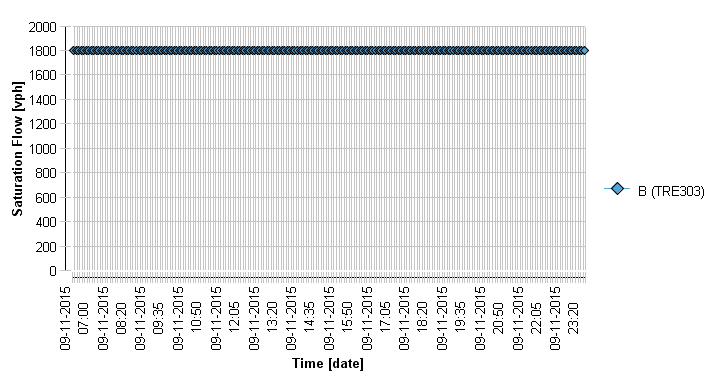
\includegraphics[height=4cm,width=0.5\linewidth]{imflowsaturation.png}
		}%
		\subfigure[Saturation flow rate]{%
			\label{fig:Saturation flow rate}
	        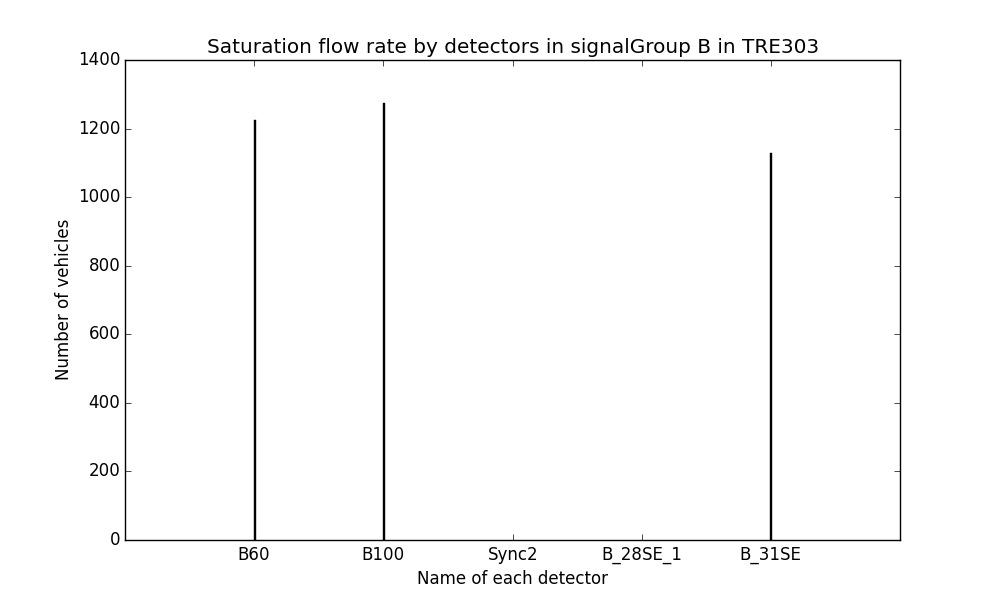
\includegraphics[height=4cm, width=0.5\linewidth]{imanalystsaturation.png}
		}\\ %  ------- End of the first row ----------------------%
	\end{center}
	\caption{%
		Queue on the four lanes
	}%
	\label{Comparison of saturation flow rate}
\end{figure}
%%%%%%% 
The reasons to cause the slight difference on green duration and volume compared with ImFlow are complicate, since the entire system is organized by many separate parts, as the flow chart ~\ref{fig:flowchart} illustrates that how the three main aspects involve into the process of traffic signal analysis service. 

First of all, every status of signals and detectors updates would be synchronous with the local data controller unit. Secondly, according to a serial of port communication between thousands of controller units and traffic flow garner system, A stream of data with information of signal, detector state and other associated attributes keeps being collected on database server.  At the Internet level, the requests are sent from front-end by traffic engineers via browser to the back end of service. When the computation using data retrieved from database completes, the content of analysis will render to web pages.

On the first step, data flow recording the status of signals and detectors is collected from numerous and independent traffic signal control units, and packed in data packets with a serial of sequence numbers. Besides, delay of information transmission is also possible to happen but immeasurable in this research. On the other hand, Packets missing through the processing of information transmission is uncontrollable. By check the sequence number of data flow from 6th to 9th of October, packet missing with one or two sequence number lost, happened about hundreds times in every day, which certainly could have influence on the analysis. On the other hand, provided that the configuration and equipment of Imflow and ImAnalyst are unequal, their reaction speed might be different and caused time lagging could effects on the edge of data set with fixed time interval. 

However, according to those comparisons of results under same parameters using ImFlow and ImAnalyst, the two kind curve lines changing match with small reasonable difference. It proves that ImAnalyst reflects the actual signal timing and the deviation is allowable in industry which have no effect on prediction of traffic capacity and examination of signals operation.

%%%%%%%%%%%%%%%%%%%%%%%%%%%%%%%%%%%%%%%%%%%%%%%%%%%%%%%%%%%%%%%%%%%%%%%%%%%%%%%%%%%%%%%%%%%%%%%%%%%%%
\section{Analysis of traffic signal measurements}
\subsection{Signal timing plan of operation}

\begin{figure}
	\hspace*{-.5in}
	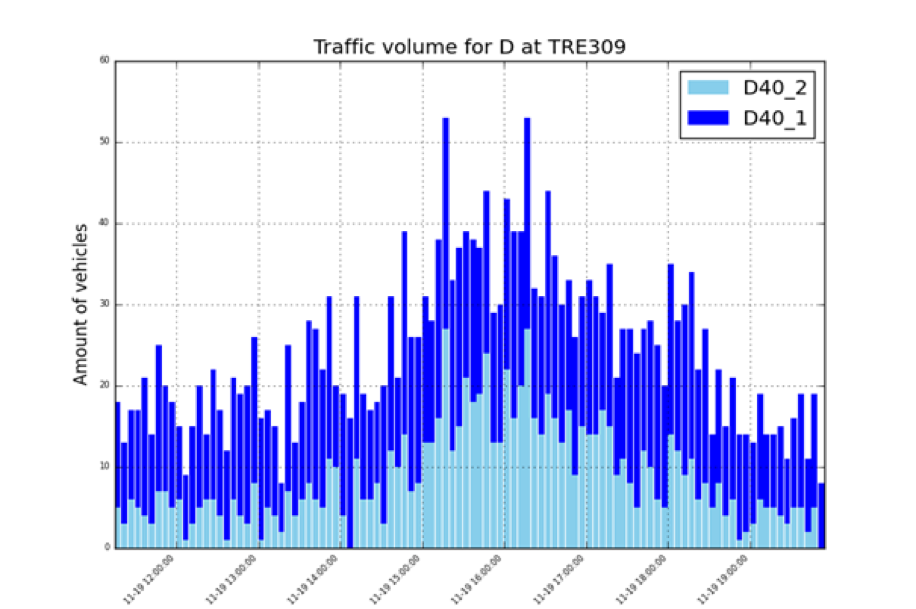
\includegraphics[width=1.2\linewidth]{planvolume.png}
	\caption{Volume by time}
	\label{fig:volume by time}
\end{figure}

The determination of signal timing plans should establish the appropriate basic timing and consider if the signal is coordinated with other nearby signals as a system or operate in isolation [~\cite{STM:2008}]. 

Different plans are used to adapt and adjust traffic on movements in different time. On 19th of November, at 18:00 a new plan replaced the previous plan for rush hour at intersection TRE309.  However, as we can see from the following figure \ref{fig:volume by time}, volume on the direction D still remained a high value in a half hour after 18 pm, even higher than that on rush time on some points. It means that if only considering the single direction, the plan changed a little bit earlier than the busy traffic flow discharging on that day and it could be improved.

The kind of indicators like traffic volume could be helpful for traffic engineers when inspect  signals work and design operation plans.  


\subsection{Green allocation} 

It is also beneficial to improve operational performance and resource allocation with analysis of signal performances measurements. Queue estimation at intersections is a significant indicator of traffic situation. The risk of cycle failure is increased with long-queued vehicles. The subfigures \ref{fig:first} and \ref{fig:second} illustrate queue on the direction controlled by signal B  at intersection TRE209 from 9:00 to 20:00, while\ref{fig:third} and \ref{fig:fourth} are for signal C. It is deduced that the level of congestion on the lanes of signal C is  significantly higher than that of signal B and longer queues generally need more time to discharge.  Besides, traffic volumes on the two directions also show that signal C faces more vehicles burden with much shorter green timing (figure \ref{fig:green duration of signal B and C at TRE209}). The allocation of signal phases is complicated but this kind of unbalance is worthy to paying attention to and reporting. 
%%%%%%% Multiple images
\begin{figure}[ht!]
	\begin{center}
		%
		\subfigure[Queue by B45 1]{%
			\label{fig:first}
			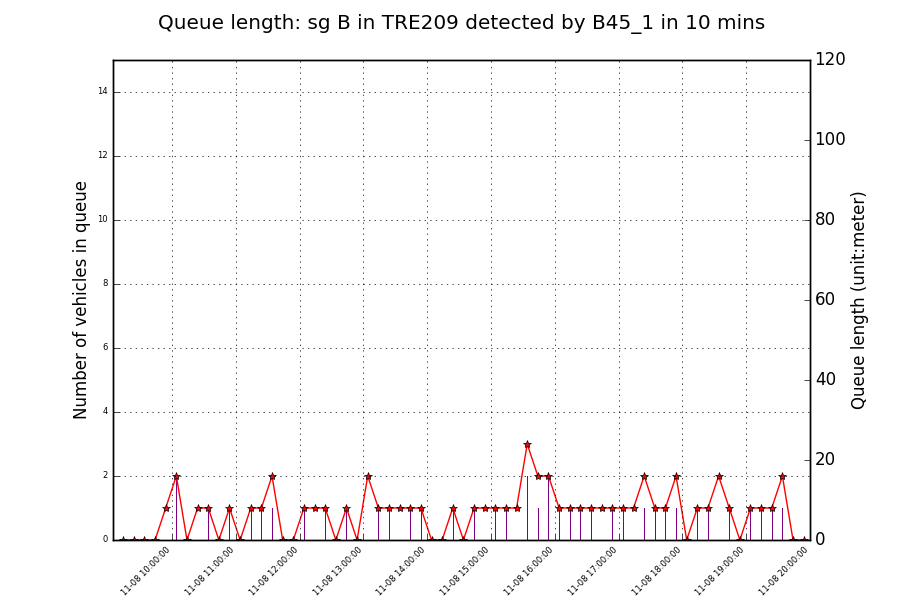
\includegraphics[width=0.4\textwidth]{b1.png}
		}%
		\subfigure[Queue by B45 2]{%
			\label{fig:second}
			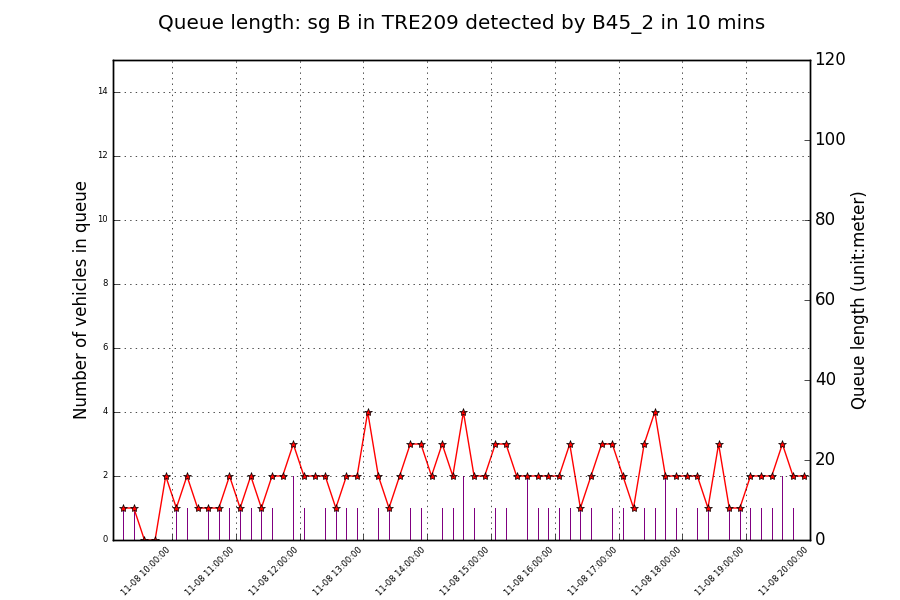
\includegraphics[width=0.4\textwidth]{b2.png}
		}\\ %  ------- End of the first row ----------------------%
		\subfigure[Queue by C50 1]{%
			\label{fig:third}
			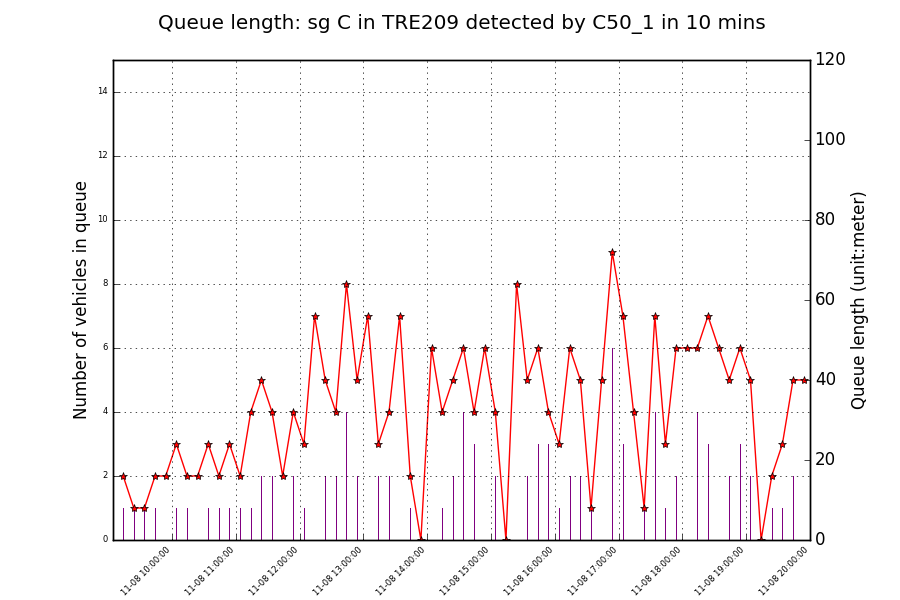
\includegraphics[width=0.4\textwidth]{c1.png}
		}%
		\subfigure[Queue by C50 2]{%
			\label{fig:fourth}
			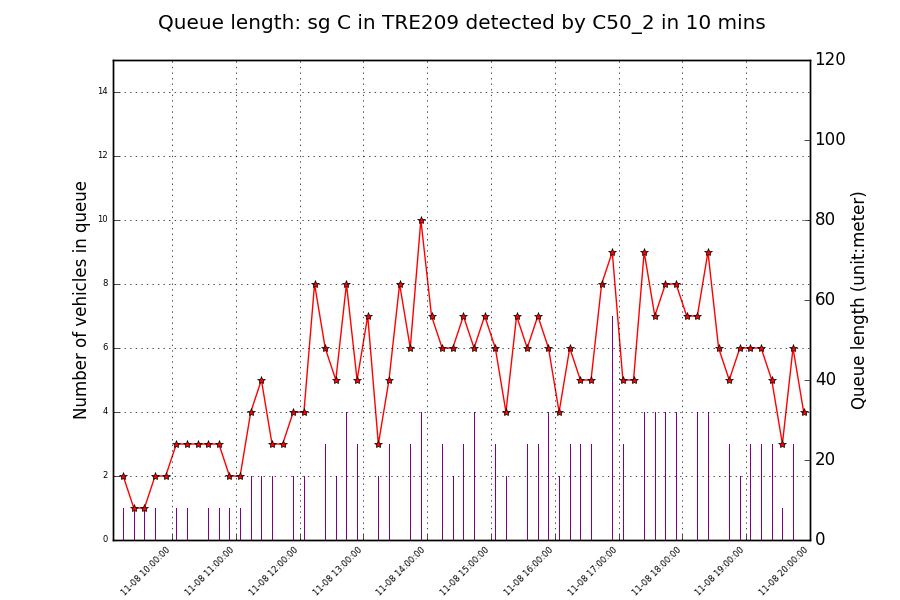
\includegraphics[width=0.4\textwidth]{c2.png}
		}%
		%
	\end{center}
	\caption{%
		Queue on the four lanes
	}%
	\label{fig:subfigures}
\end{figure}
%%%%%%% 
%%%%%%% Multiple images
\begin{figure}[ht!]
	\begin{center}
		%
		\subfigure[Green duration of signal B and C]{%
			\label{fig: green duration of signal B and C}
			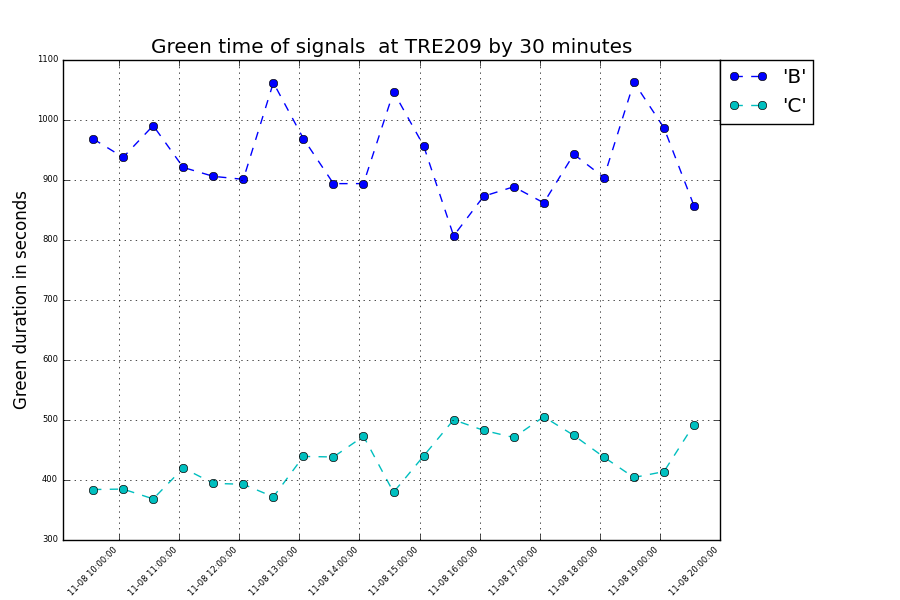
\includegraphics[height=5cm,width=0.5\linewidth]{greentre209.png}
		}%
		\subfigure[Volume of the four lanes]{%
			\label{fig: volume of the four lanes}
			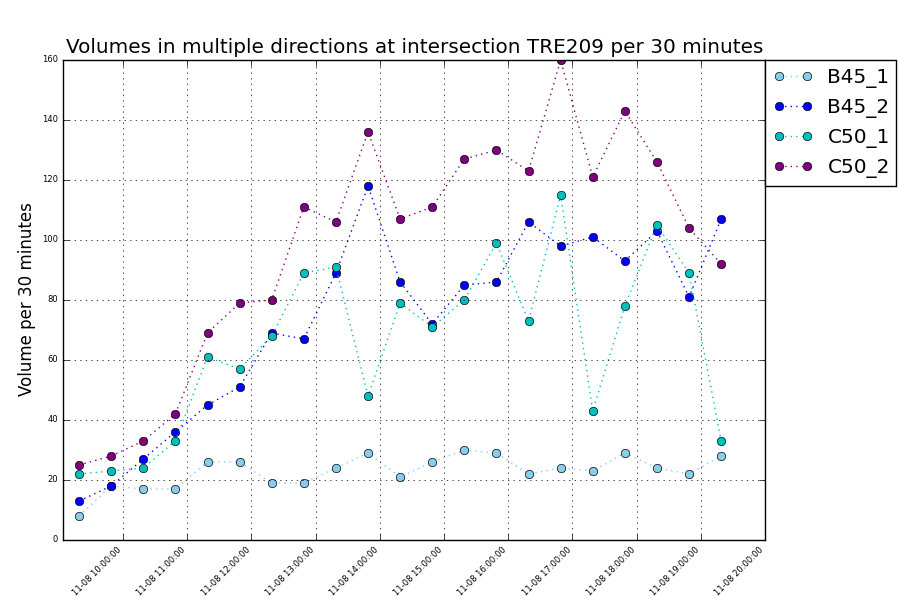
\includegraphics[height=5cm, width=0.5\linewidth]{Volumetre209.png}
		}\\ %  ------- End of the first row ----------------------%
	\end{center}
	\caption{%
		Green duration of signal B and C at TRE209
	}%
	\label{fig:green duration of signal B and C at TRE209}
\end{figure}

%%%%%%%%%%%%%%%%%%%%%%%%%%%%%%%%%%%%%%%%%%%%%%%%%%%%%%%%%%%%%%%%%%%%
\chapter{Discussion}\label{Discussion}

In this research, eight measurements of traffic signal performances are modelled and implemented and their visualized results also are represented. Three measurements of all the experiments are compared with that from ImFlow using same parameters, the professional analysis tool. The compared measurements are volume, green duration and saturation flow rate.  The results of comparison for volume and green duration demonstrate that this research gets similar analytical data with ImFlow and the visualized graphs generated by the two tools show same trend.  As for saturation flow rate, the result represents considerable difference. The reason to cause the difference is that ImFlow sets pre-defined value of saturation flow rate for every lane, while this research calculates the value using real time data, considering weather, road condition and other environment factors. When traffic is under saturated, the algorithm cannot match well.  The web-based application implemented during the research also is provided to the traffic engineers in the city of Tampere, for testing the reliability and efficiency of the application and also validating the research fundamental. The positive feedback from traffic engineers proves that research is valuable. However, as traffic signal performances are complicated, the research is still inadequate and further study and investigation will be carried out in the future. The accuracy of estimation could be improved and more measurements is expected to be implemented, like number of stops. 

%%%%%%%%%%%%%%%%%%%%%%%%%%%%%%%%%%%%%%%%%%%%%%%%%%%%%%%%%%%%%%%%%%%%
\chapter{Conclusion}
In a conclusion, the thesis provides approaches to process and analyze traffic signal data in Finland, implements and visualize measurements of traffic signal performances. An important contribution of the thesis is that provides an economical and lightweight solution to analyze traffic signal data and spreads the service to general intersections. Before that, there is some other business product in the market supporting traffic signal analysis, but it requires construction and installation on roadway and at this moment, only available in serval intersections in Tampere.  

In the chapter ~\ref{ch:The analysis and visualization}, it presents the original approaches and experimental results in detail.  In order to verify and evaluate the accuracy of experiments, the first part of the chapter  ~\ref{ch:Validation of evaluation} compares a part of experimental results with that mature product, which is currently serving ten intersections in Tampere.  The second part of chapter  ~\ref{ch:Validation of evaluation}  shows some case analysis in traffic signal research using experimental results. Definitely, there are more possibilities of traffic signal data analysis and further research is worthy of continuing. 




%%%%%%%%%%%%%%%%%%%%%%%%%%%%%%%%%%%%%%%%%%%%%%%%%%%%%%%%%%%%%%%%%%%%

\chapter{Acknowledgements}

Foremost, I would like to express my deepest gratitude to my supervisor, prof. Jyrki Nummenmaa for the continuous support to my study and research. He provided me the precious opportunity to work in the traffic analysis research group and recommended me to do the interesting and meaningful thesis work at Imtech traffic {\&} infra Oy. Those work enhanced my professional skills and gave me financial support. His guidance helps me in all the time of research and writing of the thesis. Without the work experience at traffic analysis research group, it would not be possible to conduct this thesis. I feel so fortunate to be a student of such a prestigious and farsighted professor. 

My sincere thanks also go to all my colleagues in Imtech Oy. They always tried their best to help me and answer my questions related to my work.  In particular,  Mr. Jukka-Pekka Alanissi, my boss and the regional manager of Imtech Oy, who wisely created the project of traffic signal analysis and hired me work for my thesis in the project.  And I sincerely thank Mr. Petri Ahola, who is an experienced and skilful software engineer. Petri mentored my work at the company, gave me guidance and insightful comments on programming, also taught me professional knowledge on traffic engineering in Finland patiently. I learned a lot from him about how to be a qualified software developer and knew that programming is hard but fun.

I am also grateful to all the people helped me during my study in University of Tampere, Paula Syrj�rinne and Timo Nummenmaa in the traffic analysis research group encouraged and inspired my research at this field.  I also thankful to my lab mates, especially Elena Betekhtina, she helped me to enrich my ideas on my research, commented on my views and shared useful information with me. I spent good time with them. I would like to acknowledge all the teachers taught me in UTA, especially Prof. Zhang Zheying for numerous lectures about thesis and good suggestions to me. She is one of the best teachers I have met here and cares every student. 

Many friends help me and concern me. I greatly value their friendship and appreciate their belief in me. They brought a lot of happiness and precious memories to me. Once I got in trouble, they always stand on me and support me. My friends helped me move apartments three times, which I cannot imagine how to deal with it by myself; we celebrated every traditional Chinese holiday together and they let me not feel lonely or isolated while studying aboard; they made a fancy double-heart cake and surprised me on my birthday.... They are not only my friends, they are also my families in Finland. 

Most importantly, none of this would have been possible without the love and support from my family. The thesis is dedicated to them who give me unconditional and constant love, concern and support all these years. I would like to express my heart-felt gratitude to my parents. And the person who gives me most support is my loving fianc�, Song Ji, who helped me overcome setbacks in the most difficulty time of thesis work, who encourages me to believe and fulfil myself, who accompanies me at every moment of happiness and sadness in the past five years... It would take days to tell it all. I am certainly imperfect person but I meet the perfect love. I desire to create our future with the best man. 

%%%%%%%%%%%%%%%%%%%%%%%%%%%%%%%%%%%%%%%%%%%%%%%%%%%%%%%%%%%%%%%%%%%%

% You can add text to the beginning of the list of references with natbib's command \bibpreamble:
\renewcommand{\bibpreamble}{\par\medskip}

% When using BibTeX, the environment thebibliography must be replaced with the following two commands:
\bibliographystyle{utastmth}

\bibliography{viitteet} 


%%%%%%%%%%%%%%%%%%%%%%%%%%%%%%%%%%%%%%%%%%%%%%%%%%%%%%%%%%%%%%%%%%%%
% The appendices will be numbered:
\appendix
% but if there is only one appendix, it will not be numbered.
\setcounter{secnumdepth}{-2}

% If the appendix is made with some other program, it can be included to the thesis as a pdf-file using the command \includepdf from pdfpages package:
%\includepdf[pages={1-4}]{filename.pdf}

%\chapter{Appendix: Using \BibTeX}\label{ch: Using BibTeX}




%%%%%%%%%%%%%%%%%%%%%%%%%%%%%%%%%%%%%%%%%%%%%%%%%%%%%%%%%%%%%%%%%%%%
% If the thesis contains an index, it will be placed here:
%\printindex


\end{document}
%%%%%%%%%%%%%%%%%%%%%%%%%%%%%%%%%%%%%%%%%%%%%%%%%%%%%%%%%%%%%%%%%%%%